\begin{table}
   \begin{subtable}[h]{1\textwidth}
    \small
   \begin{tabular}{|l|p{5.5cm}|l|l|}

\hline

\bf{Version} & \bf {Contexte} & \bf{\texttt{spaCy\_lg}}&\bf{\texttt{stanza}}\\
\hline

Réf.\ & \textit{[...] rue de Sèvres ;}&rue de Sèvres
 & rue de Sèvres \\

Kraken & \textit{[...] ru\textcolor{red}{c} de S\textcolor{red}{b}vr\textcolor{red}{c}s ;} & \textbf{\_} S\textcolor{red}{b}vr\textcolor{red}{c}s &  \textbf{\_} S\textcolor{red}{b}vr\textcolor{red}{c}s \\ 

Tess & \textit{[...] rue de S\textcolor{red}{é}vres;}& \textbf{\_} S\textcolor{red}{é}vres &  rue de S\textcolor{red}{é}vres\\
Tess fr &  \textit{[...]  rue de Sèvres ;} & rue de Sèvres & rue de Sèvres\\
\hline % ajout des exemples de la TGB
%Réf. & \textit{ [...] le faubourg Saint-Germain} &faubourg  Saint-Germain&faubourg Saint-Germain \\
 %Kraken &\textit{[...] l\textcolor{red}{c} faubourg Saint-G\textcolor{red}{c}rmain} &\textbf{\_}Saint-G\textcolor{red}{c}rmain&  faubourg Saint-G\textcolor{red}{c}rmain \\ 
 %Tess & \textit{[...] le faubourg Saint-Germain}&  faubourg Saint-Germain & faubourg Saint-Germain \\
%Tess fr &\textit{[...] le faubourg Saint-Germain}&  faubourg Saint-Germain &  faubourg Saint-Germain \\
%\hline

Réf.\ & \textit{[...] dans la Ville de Brundu\textcolor{red}{f}ie} & \textcolor{red}{()}& Ville deBrundu\textcolor{red}{f}ie\\
 Kraken &\textit{[...] dans la Ville de Brundu\textcolor{red}{t}ie} &Ville de Brundu\textcolor{red}{t}ie & Ville de  Brundu\textcolor{red}{t}ie \\ 
 Tess & \textit{[...] dans la Ville de Brundu\textcolor{red}{f}ie} & \textcolor{red}{()} &Ville de Brundu\textcolor{red}{f}ie  \\
Tess fr & \textit{[...] dans la Ville de Brundu\textcolor{red}{f}ie} & \textcolor{red}{()} & Ville de Brundu\textcolor{red}{f}ie \\
\hline
\end{tabular}



    \caption{Pontmartin et Bourdeille (TGB).} 
    \label{tab:erreur_tgb}
    \end{subtable}

    \begin{subtable}[h]{1\textwidth}
    \small
   \resizebox{\textwidth}{!}{
\begin{tabular}{|l|p{6.7cm}|l|l|}

\hline

\bf{Version} & \bf {Contexte} & \bf{\texttt{spaCy\_lg}}&\bf{\texttt{stanza}}\\
\hline

Réf.\ & \textit{[...] il en est tombé au sort cinq de Saint-Brunelle.} & Saint-Brunelle&Saint-Brunelle  \\

Kraken &\textit{[...] il en est tombe au sort cinq
de Sain\textcolor{red}{l}-Brun\textcolor{red}{c}lle.} & Sain\textcolor{red}{l}-Brun\textcolor{red}{c}lle & Sain\textcolor{red}{l}-Brun\textcolor{red}{c}lle \\ 

Tess & \textit{[...] il en est tombé au sort cinq\textcolor{red}{'} de Saint-Brunelle.}& Saint-Brunelle&Saint-Brunelle \\
Tess fr & \textit{[...] il en est tombé au sort cinq \textcolor{red}{'} de Saint-Brunelle.}  &Saint-Brunelle &Saint-Brunelle \\
\hline 
Réf.\ & \textit{Quand, à côté de cela, la Picardie, [...]} & Picardie&  Picardie\\
 Kraken & \textit{Quand, \textcolor{red}{h} c\textcolor{red}{\_}te de
cela, la Pic\textcolor{red}{s}rdie, [...]}&Pic\textcolor{red}{s}rdie & Pic\textcolor{red}{s}rdie\\ 
 Tess &\textit{Quand, a c \textcolor{red}{d}té de cela, la Picardie, [...]} & Picardie & Picardie  \\
Tess fr &\textit{Quand, à côté de cela , la Picardie,  [...]} & Picardie  &  Picardie \\
\hline 

\end{tabular}
}
    \caption{ Adam et Carraud (ELTeC français).\label{tab:erreur_eltecfra}} 
    \end{subtable}

\begin{subtable}[h]{1\textwidth}
\small
   \begin{tabular}{|l|p{7.5cm}|l|l|}

\hline

\bf{Version} & \bf {Contexte} & \bf{\texttt{spaCy\_lg}}&\bf{\texttt{stanza}}\\
\hline

Réf.\ &\textit{There are some fields near Manchester [...] }& Manchester &Manchester  \\

Kraken & \textit{\_ are some fields near ancehester [...]}& ancehester & \textcolor{red}{()} \\ 

Tess & \textit{Non transcrit} & N/A&N/A \\

\hline 
Réf.\ & \textit{[...] then on a visit at Kilmarnock Abbey, near
     Edinburgh.} & Edinburgh &Edinburgh \\
 Kraken &\textit{[...] then on a visit at Kilmarno\textcolor{red}{e}k Abbey, near
Edinburg\textcolor{red}{l}.} & Edinburg\textcolor{red}{l} & Edinburg\textcolor{red}{l}\\ 
 Tess &\textit{[...] then on a visit at Kilmarnock Abbey, near
Edinburgh. }& Edinburgh & Edinburgh \\


\hline 

\end{tabular}

    \caption{Gaskell et Sinclair (ELTeC anglais).\label{tab:erreurs_OCR_ELTeCEng}} 
    \end{subtable}
    
    \begin{subtable}[h]{1\textwidth}
    \small
   \begin{tabular}{|l|p{7.5cm}|l|r|}

\hline

\bf{Version} & \bf {Contexte} & \bf{\texttt{spaCy\_lg}}&\bf{\texttt{stanza}}\\
\hline

Réf.\ & \textit{[...] durante todo o tempo em que estivesse em Portugal.}& Portugal& N/A \\

Kraken &\textit{[...] durant\textcolor{red}{a} todo o t\textcolor{red}{o}mpe
em q\textcolor{red}{n}e ostivess\textcolor{red}{o} em Port\textcolor{red}{n}gal.} & Port\textcolor{red}{n}gal & N/A \\ 
 Tess & \textit{[...] durante todo o tempo
em que estivess\textcolor{red}{o} em Portugal.} &Portugal  & N/A \\
Tess pt & \textit{[...] durante todo o tempo
em que estivess\textcolor{red}{o} em Portugal.}  &Portugal & N/A\\
\hline 
Réf.\ & \textit{O Crime do Padre Amaro recebeu no Bra\textcolor{red}{z}il [...] } &Bra\textcolor{red}{z}il &N/A \\
 Kraken &\textit{\textcolor{red}{\_} C\textcolor{red}{\_}I\textcolor{red}{\_}E Do PADRE A\textcolor{red}{I}ARO recebeu no Bras\textcolor{red}{lc} [...] } &Bras\textcolor{red}{lc} & N/A\\ 
 Tess &\textit{\textcolor{red}{\_} CRIME DO PADRE AMARO recebeu no Brasil [...] } &  Brasil& N/A \\
Tess pt &\textit{O\textcolor{red}{\_}RIME DO PADRE AMARO recebeu no Brasil [...] } & Brasil & N/A \\

\hline 

\end{tabular}

    \caption{Castro Osorio et Queiroz (ELTeC portugais).\label{tab:erreur_eltecpor}} 
\end{subtable}
    
    \caption{Alignement : Faux Positif ou Vrai Positif ?}
\end{table}


%______INTERSECTIONS
%____TROLLOPE
% \begin{figure}
% \begin{minipage}{7cm}
%   \begin{subfigure}{0.99\textwidth}
%   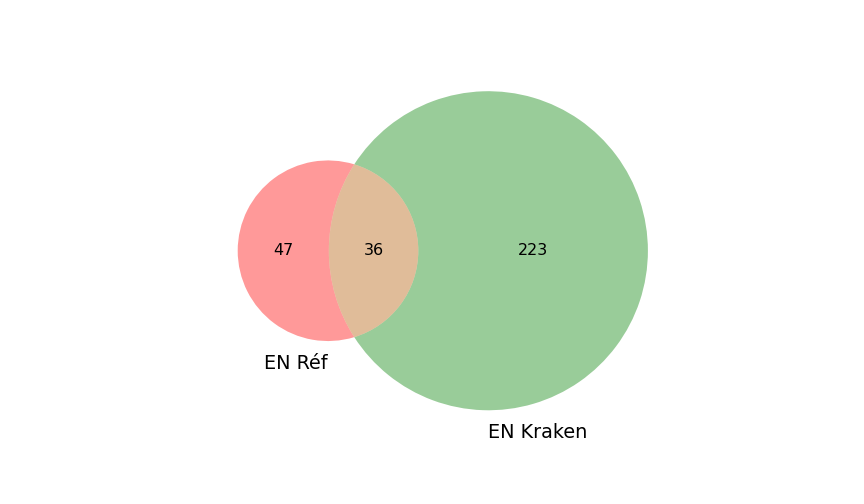
\includegraphics[width=.99\textwidth]{IMAGES/ELTeC_INTERSECTIONS_spaCy3.5.1/TROLLOPE_Adventure_Kraken.txt_spacy-lg-concat.json_intersection.png} 
%   \caption{Kraken-\textsc{spaCy\_lg}}
%   \label{fig:TROLLOP_DIST_KRAKENBASE_LG}
%   \end{subfigure}
%   \end{minipage}
%   %
%   \begin{minipage}{7cm}
%   \begin{subfigure}{0.99\textwidth}
%   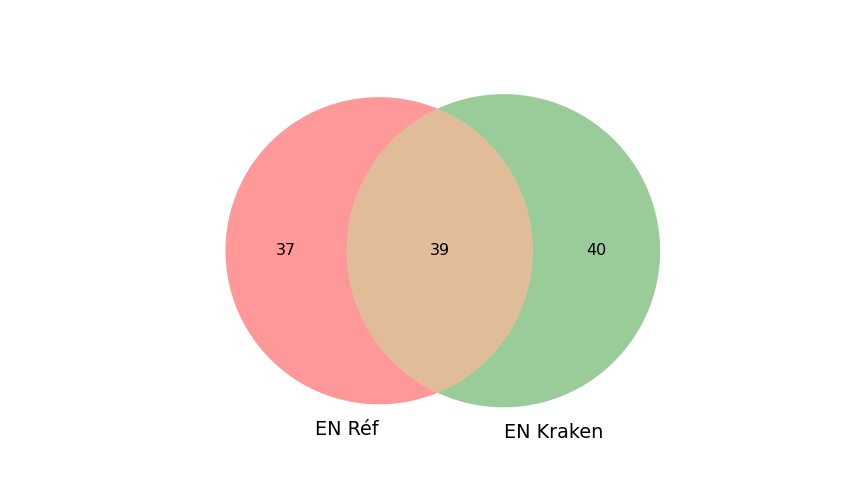
\includegraphics[width=.99\textwidth]{IMAGES/ELTeC_INTERSECTIONS_stanza/TROLLOPE_Adventure_Kraken.txt_stanza-concat.json_intersection.png}
%    \caption{Kraken-\textsc{Stanza}}
 
%   \label{fig: }
%   \end{subfigure}
%   \end{minipage}
%   %%
% %\caption{}
% %\label{fig:INTERSECTION_NOAILLES}
% %% [heigH=4cm] enlevé--> passe mal sur ACM
%   \begin{minipage}{7cm}
%   \begin{subfigure}{0.99\textwidth}
%   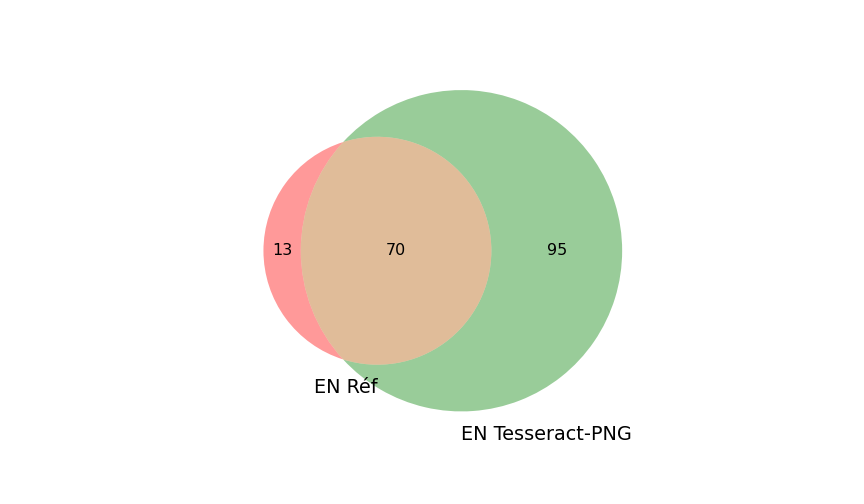
\includegraphics[width=.99\textwidth]{IMAGES/ELTeC_INTERSECTIONS_spaCy3.5.1/TROLLOPE_Adventure_Tesseract-PNG.txt_spacy-lg-concat.json_intersection.png} 
%   \caption{Tesseract-\textsc{spacy\_lg}}
%   \label{fig:}
%   \end{subfigure}
%     \end{minipage}
%   %
%   \begin{minipage}{7cm}
%   \begin{subfigure}{0.99\textwidth}
%   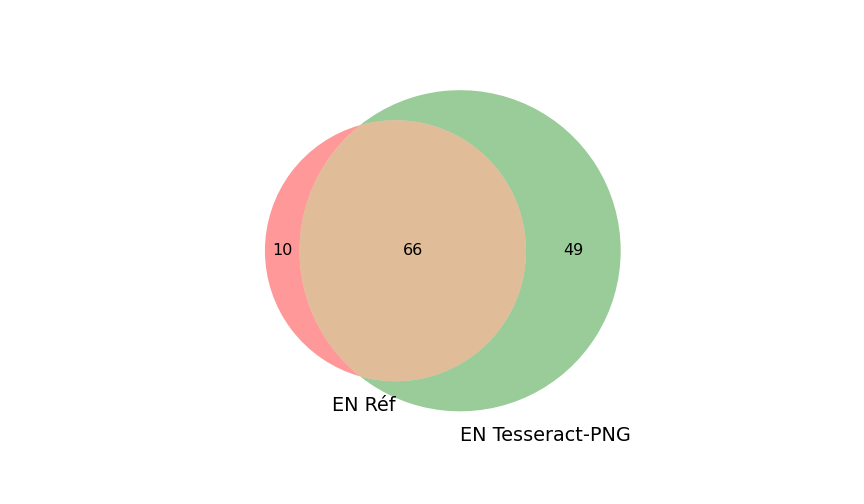
\includegraphics[width=.99\textwidth]{IMAGES/ELTeC_INTERSECTIONS_spaCy3.5.1/TROLLOPE_Adventure_Tesseract-PNG.txt_stanza-concat.json_intersection.png}
%    \caption{Tesseract-\textsc{Stanza}}
%   \label{fig: }
%   \end{subfigure}
%   \end{minipage}
% \caption{Intersections entre les EN (\texttt{spaCy\_lg, Stanza}) issues des textes de référence et des versions OCR (Kraken et Tesseract) -- Frances Trolloppe, \textit{The Life and Adventures of M. Armstrong} ; exemple d'un bon OCR, corpus ELTeC anglais.}
% \label{fig:}
% \end{figure}

%____BRONTË
% \begin{figure}
% \begin{minipage}{7cm}
%   \begin{subfigure}{0.99\textwidth}
%   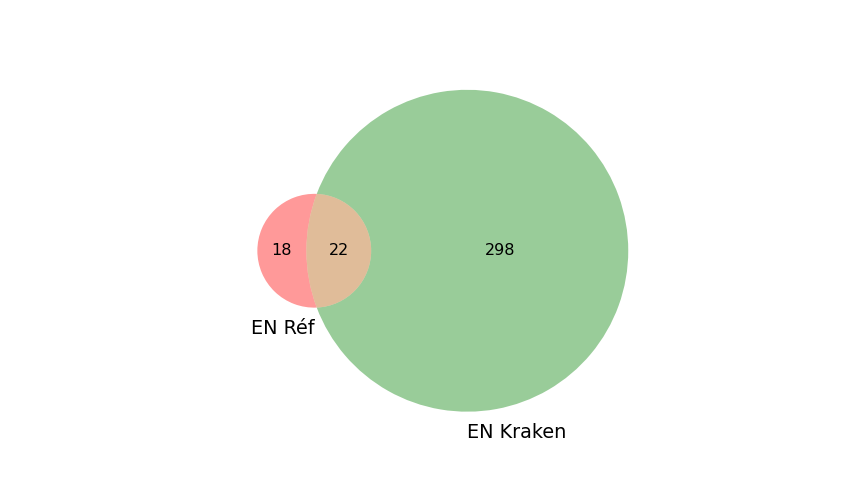
\includegraphics[width=.99\textwidth]{IMAGES/ELTeC_INTERSECTIONS_spaCy3.5.1/BRONTE_Wuthering-heights_Kraken.txt_spacy-lg-concat.json_intersection.png} 
%   \caption{Kraken-\textsc{spaCy\_lg}}
%   \label{fig:TROLLOP_DIST_KRAKENBASE_LG}
%   \end{subfigure}
%   \end{minipage}
%   %
%   \begin{minipage}{7cm}
%   \begin{subfigure}{0.99\textwidth}
%   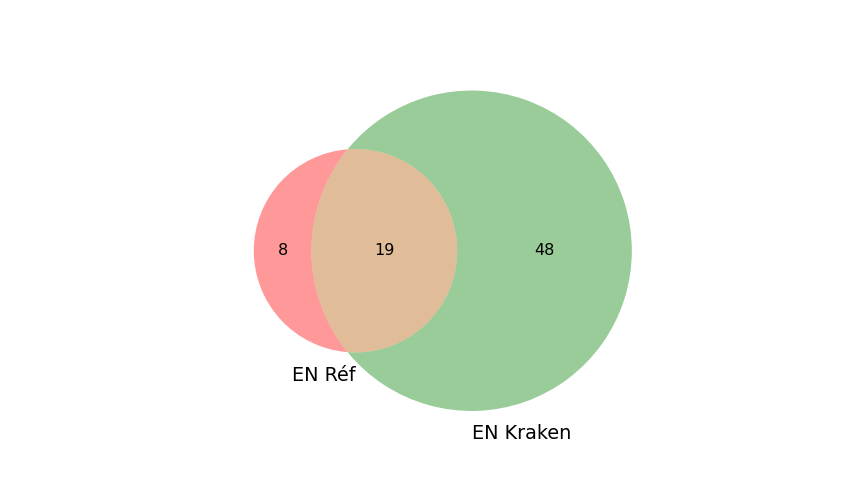
\includegraphics[width=.99\textwidth]{IMAGES/ELTeC_INTERSECTIONS_stanza/BRONTE_Wuthering-heights_Kraken.txt_stanza-concat.json_intersection.png}
%    \caption{Kraken-\textsc{stanza}}
 
%   \label{fig: }
%   \end{subfigure}
%   \end{minipage}
%   %%
% %\caption{}
% %\label{fig:INTERSECTION_NOAILLES}
% %% [heigH=4cm] enlevé--> passe mal sur ACM
%   \begin{minipage}{7cm}
%   \begin{subfigure}{0.99\textwidth}
%   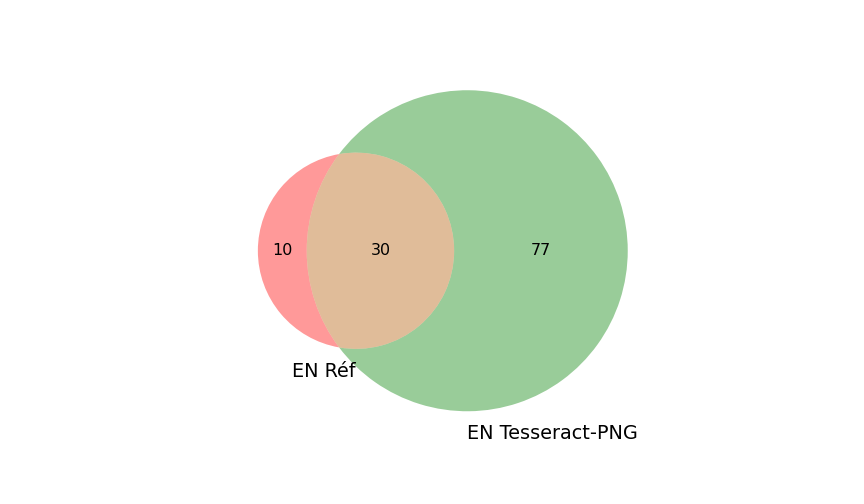
\includegraphics[width=.99\textwidth]{IMAGES/ELTeC_INTERSECTIONS_spaCy3.5.1/BRONTE_Wuthering-heights_Tesseract-PNG.txt_spacy-lg-concat.json_intersection.png} 
%   \caption{Tesseract-\textsc{spacy\_lg}}
%   \label{fig:}
%   \end{subfigure}
%     \end{minipage}
%   %
%   \begin{minipage}{7cm}
%   \begin{subfigure}{0.99\textwidth}
%   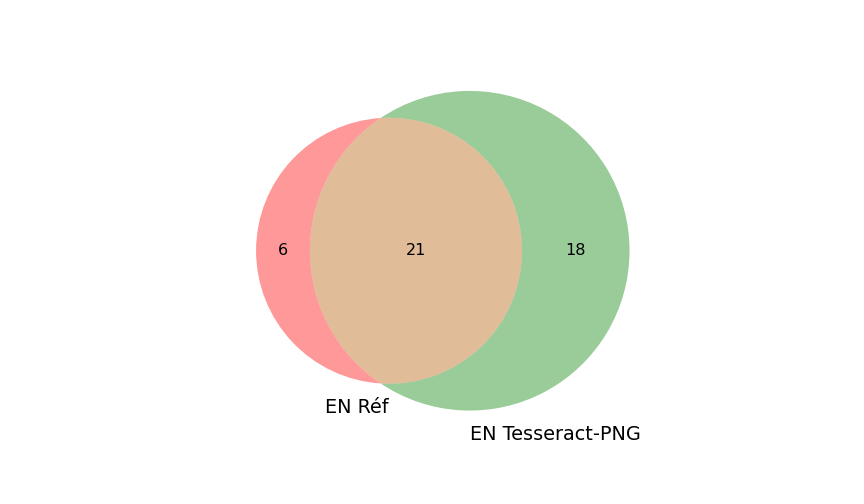
\includegraphics[width=.99\textwidth]{IMAGES/ELTeC_INTERSECTIONS_stanza/BRONTE_Wuthering-heights_Tesseract-PNG.txt_stanza-concat.json_intersection.png}
%    \caption{Tesseract-\textsc{stanza}}
%   \label{fig: }
%   \end{subfigure}
%   \end{minipage}
% \caption{Intersections entre les EN (spaCy\_lg, stanza) issues des textes de référence et des versions OCR (Kraken et Tesseract) -- Emily Brontë, \textit{Wuthering HeigHs}.}
% \label{fig:}
% \end{figure}

%____REYNOLDS
% \begin{figure}
% \begin{minipage}{7cm}
%   \begin{subfigure}{0.99\textwidth}
%   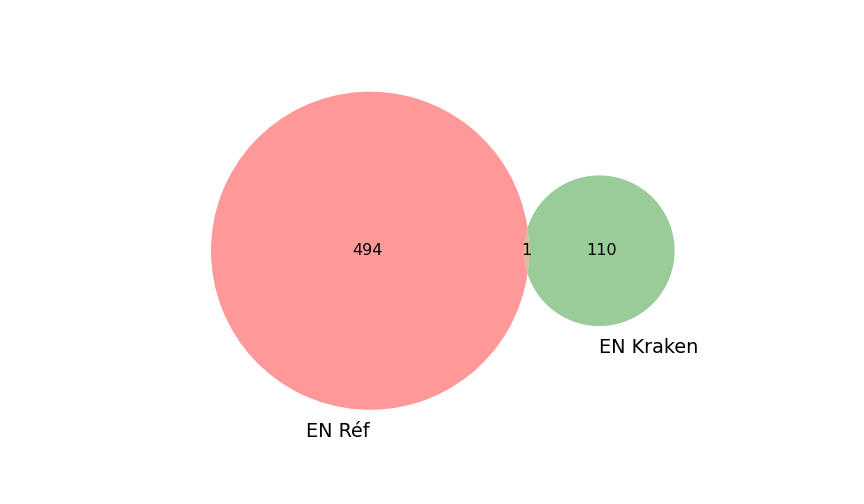
\includegraphics[width=.99\textwidth]{IMAGES/ELTeC_INTERSECTIONS_spaCy3.5.1/REYNOLDS_The-Mysteries-of-London_Kraken.txt_spacy-lg-concat.json_intersection.png} 
%   \caption{Kraken-\textsc{spaCy\_lg}}
%   \label{fig:TROLLOP_DIST_KRAKENBASE_LG}
%   \end{subfigure}
%   \end{minipage}
%   %
%   \begin{minipage}{7cm}
%   \begin{subfigure}{0.99\textwidth}
%   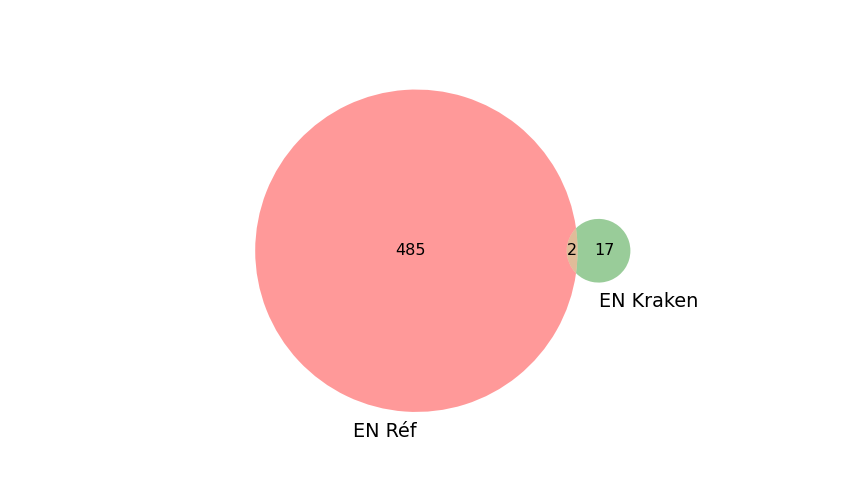
\includegraphics[width=.99\textwidth]{IMAGES/ELTeC_INTERSECTIONS_stanza/REYNOLDS_The-Mysteries-of-London_Kraken.txt_stanza-concat.json_intersection.png}
%    \caption{Kraken-\textsc{Stanza}}
 
%   \label{fig: }
%   \end{subfigure}
%   \end{minipage}
%   %%
% %\caption{}
% %\label{fig:INTERSECTION_NOAILLES}
% %% [heigH=4cm] enlevé--> passe mal sur ACM
%   \begin{minipage}{7cm}
%   \begin{subfigure}{0.99\textwidth}
%   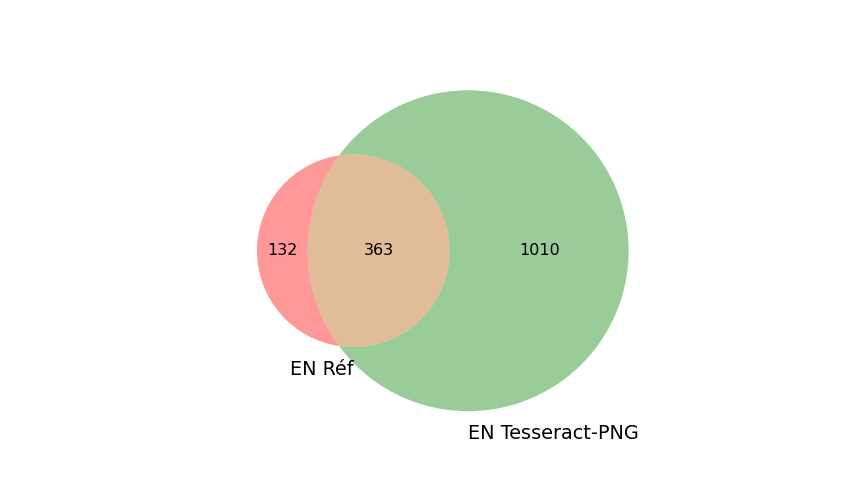
\includegraphics[width=.99\textwidth]{IMAGES/ELTeC_INTERSECTIONS_spaCy3.5.1/REYNOLDS_The-Mysteries-of-London_Tesseract-PNG.txt_spacy-lg-concat.json_intersection.png} 
%   \caption{Tesseract-\textsc{spacy\_lg}}
%   \label{fig:}
%   \end{subfigure}
%     \end{minipage}
%   %
%   \begin{minipage}{7cm}
%   \begin{subfigure}{0.99\textwidth}
%   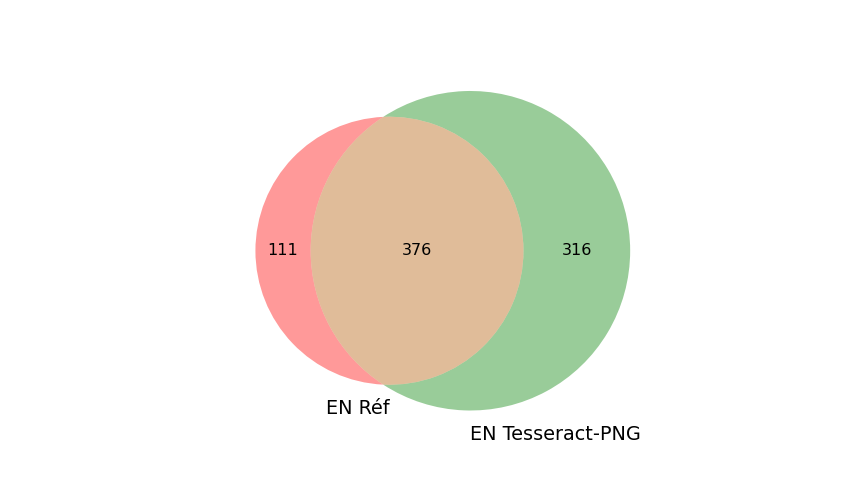
\includegraphics[width=.99\textwidth]{IMAGES/ELTeC_INTERSECTIONS_stanza/REYNOLDS_The-Mysteries-of-London_Tesseract-PNG.txt_stanza-concat.json_intersection.png}
%    \caption{Tesseract-\textsc{Stanza}}
%   \label{fig: }
%   \end{subfigure}
%   \end{minipage}
% \caption{Intersections entre les EN (\texttt{spaCy\_lg, stanza}) issues des textes de référence et des versions OCR (Kraken et Tesseract) -- G. W. M. Reynolds, \textit{The Mysteries of London} ; exemple d'un mauvais OCR, corpus ELTeC anglais.}
% \label{fig:}
% \end{figure}

%____MAUPASSANT
% \begin{figure}
% \begin{minipage}{7cm}
%   \begin{subfigure}{0.99\textwidth}
%   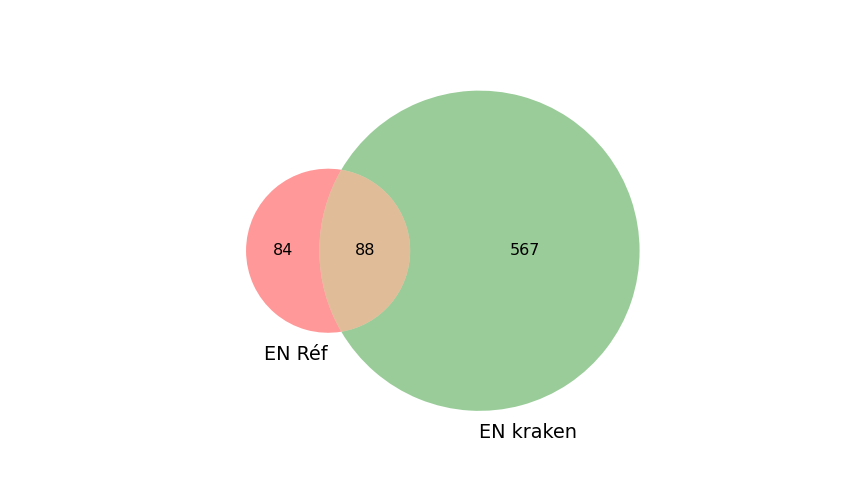
\includegraphics[width=.99\textwidth]{IMAGES/ELTeC_INTERSECTIONS_spaCy3.5.1/MAUPASSANT_une-vie_Kraken-base.txt_spacy-lg-concat.json_intersection.png} 
%   \caption{Kraken-\textsc{spaCy\_lg}}
%   \label{fig:TROLLOP_DIST_KRAKENBASE_LG}
%   \end{subfigure}
%   \end{minipage}
%   %
%   \begin{minipage}{7cm}
%   \begin{subfigure}{0.99\textwidth}
%   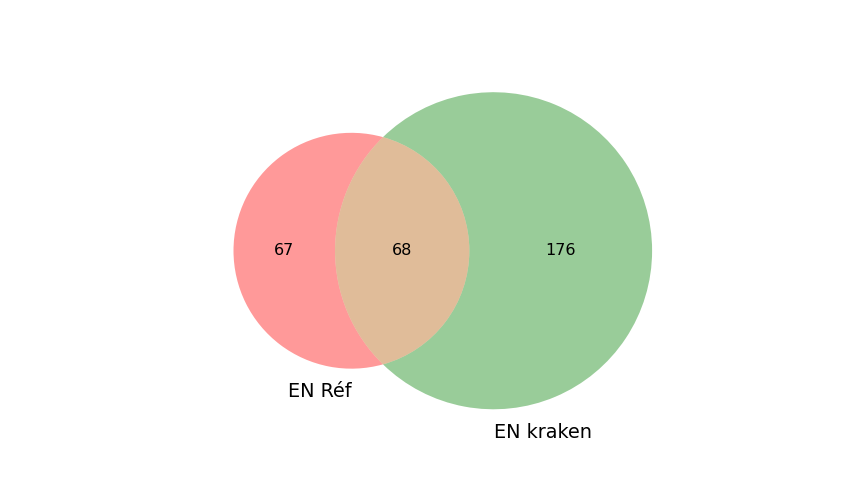
\includegraphics[width=.99\textwidth]{IMAGES/ELTeC_INTERSECTIONS_stanza/MAUPASSANT_une-vie_Kraken-base.txt_stanza-concat.json_intersection.png}
%    \caption{Kraken-\textsc{stanza}}
 
%   \label{fig: }
%   \end{subfigure}
%   \end{minipage}
%   %%
% %\caption{}
% %\label{fig:INTERSECTION_NOAILLES}
% %% [heigH=4cm] enlevé--> passe mal sur ACM
%   \begin{minipage}{7cm}
%   \begin{subfigure}{0.99\textwidth}
%   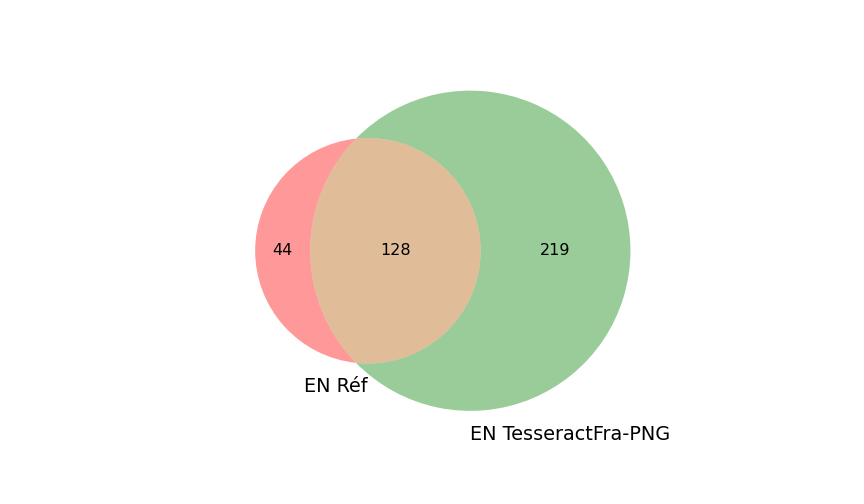
\includegraphics[width=.99\textwidth]{IMAGES/ELTeC_INTERSECTIONS_spaCy3.5.1/MAUPASSANT_une-vie_TesseractFra-PNG.txt_spacy-lg-concat.json_intersection.png} 
%   \caption{Tesseract-\textsc{spacy\_lg}}
%   \label{fig:}
%   \end{subfigure}
%     \end{minipage}
%   %
%   \begin{minipage}{7cm}
%   \begin{subfigure}{0.99\textwidth}
%   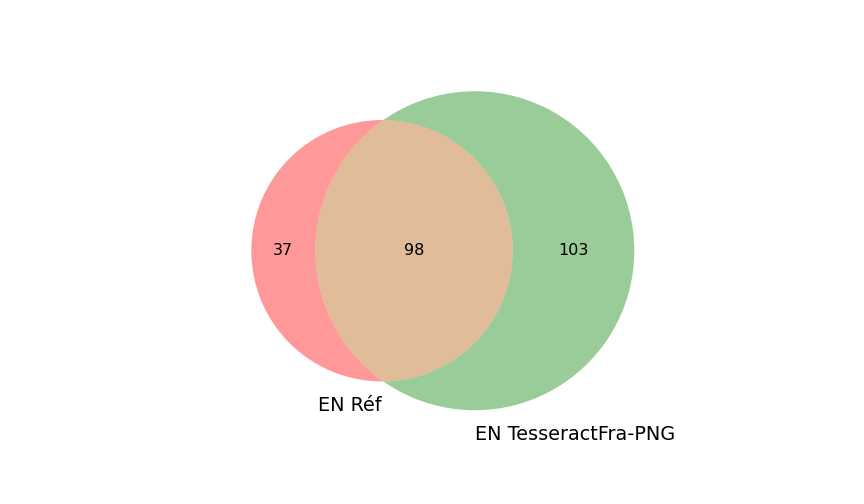
\includegraphics[width=.99\textwidth]{IMAGES/ELTeC_INTERSECTIONS_stanza/MAUPASSANT_une-vie_TesseractFra-PNG.txt_stanza-concat.json_intersection.png}
%    \caption{Tesseract-\textsc{stanza}}
%   \label{fig: }
%   \end{subfigure}
%   \end{minipage}
% \caption{Intersections entre les EN (spaCy\_lg, stanza) issues des textes de référence et des versions OCR (Kraken et Tesseract) -- Guy de Maupassant, \textit{Une vie}.}
% \label{fig:}
% \end{figure}



%____ADAM
% \begin{figure}
% \begin{minipage}{7cm}
%   \begin{subfigure}{0.99\textwidth}
%   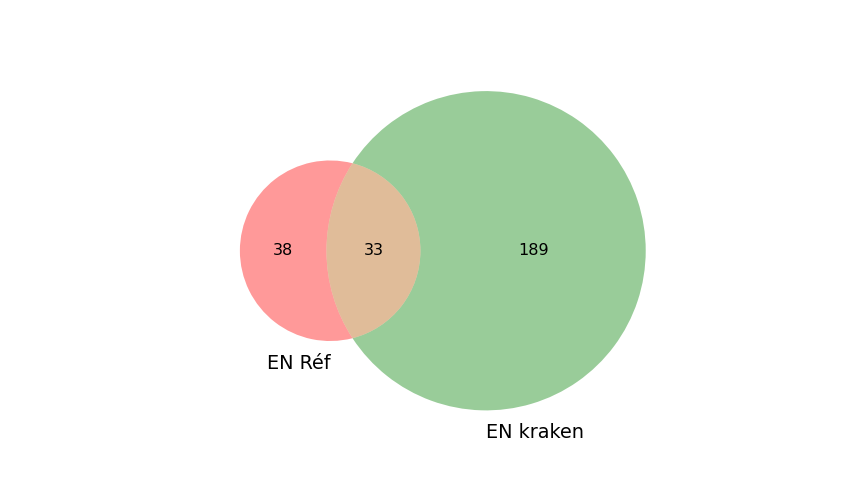
\includegraphics[width=.99\textwidth]{IMAGES/ELTeC_INTERSECTIONS_spaCy3.5.1/ADAM_Mon-village_Kraken-base.txt_spacy-lg-concat.json_intersection.png} 
%   \caption{Kraken-\textsc{spaCy\_lg}}
%   \label{fig:TROLLOP_DIST_KRAKENBASE_LG}
%   \end{subfigure}
%   \end{minipage}
%   %
%   \begin{minipage}{7cm}
%   \begin{subfigure}{0.99\textwidth}
%   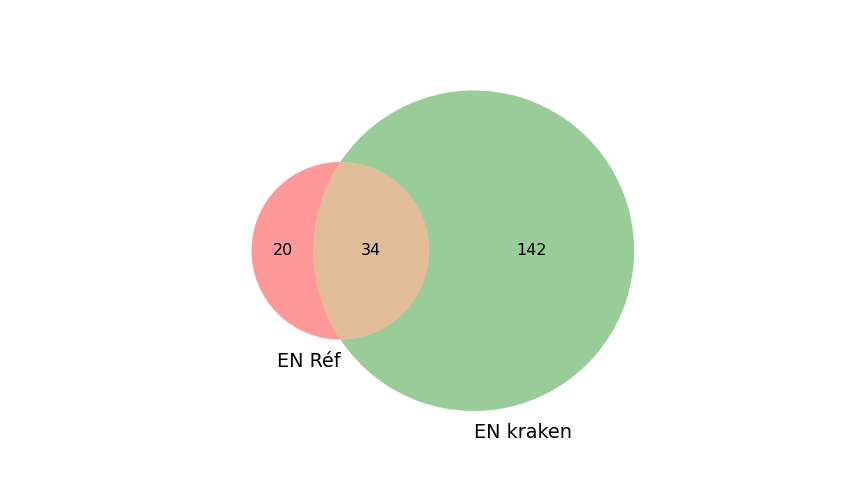
\includegraphics[width=.99\textwidth]{IMAGES/ELTeC_INTERSECTIONS_stanza/ADAM_Mon-village_Kraken-base.txt_stanza-concat.json_intersection.png}
%    \caption{Kraken-\textsc{stanza}}
 
%   \label{fig: }
%   \end{subfigure}
%   \end{minipage}
%   %%
% %\caption{}
% %\label{fig:INTERSECTION_NOAILLES}
% %% [heigH=4cm] enlevé--> passe mal sur ACM
%   \begin{minipage}{7cm}
%   \begin{subfigure}{0.99\textwidth}
%   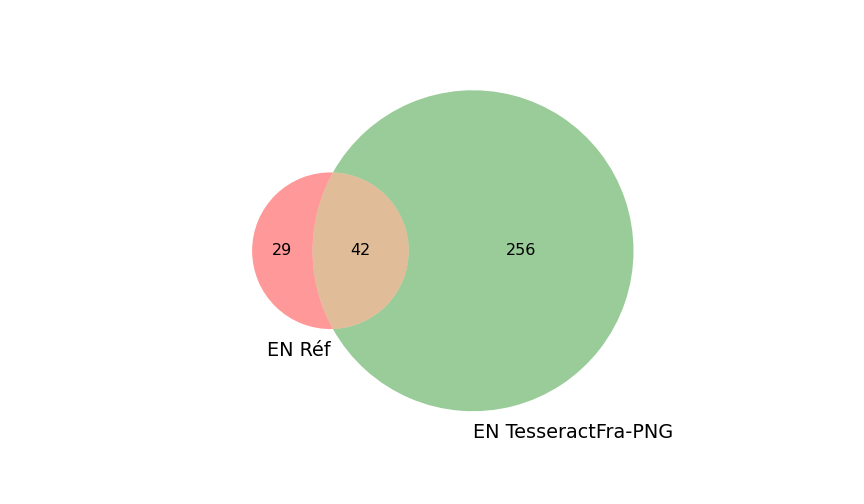
\includegraphics[width=.99\textwidth]{IMAGES/ELTeC_INTERSECTIONS_spaCy3.5.1/ADAM_Mon-village_TesseractFra-PNG.txt_spacy-lg-concat.json_intersection.png} 
%   \caption{Tesseract-\textsc{spacy\_lg}}
%   \label{fig:}
%   \end{subfigure}
%     \end{minipage}
%   %
%   \begin{minipage}{7cm}
%   \begin{subfigure}{0.99\textwidth}
%   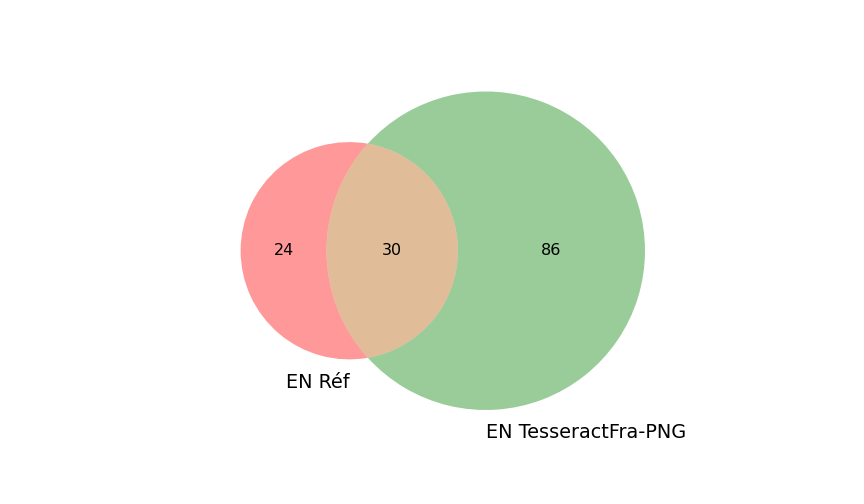
\includegraphics[width=.99\textwidth]{IMAGES/ELTeC_INTERSECTIONS_stanza/ADAM_Mon-village_TesseractFra-PNG.txt_stanza-concat.json_intersection.png}
%    \caption{Tesseract-\textsc{stanza}}
%   \label{fig: }
%   \end{subfigure}
%   \end{minipage}
% \caption{Intersections entre les EN (\texttt{spaCy\_lg, stanza}) issues des textes de référence et des versions OCR (Kraken et Tesseract) -- Juliette Adam (Lambert), \textit{Mon village} ; exemple d'un mauvais OCR, corpus ELTeC français.}
% \label{fig:}
% \end{figure}



%____CASTRO-OSORIO
% \begin{figure}
% \begin{minipage}{7cm}
%   \begin{subfigure}{0.99\textwidth}
%   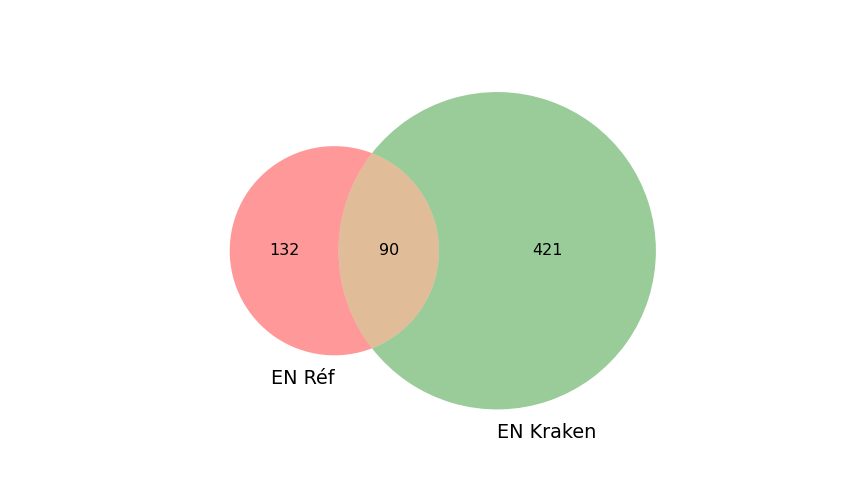
\includegraphics[width=.99\textwidth]{IMAGES/ELTeC_INTERSECTIONS_spaCy3.5.1/CASTRO-OSORIO_quatro-novelas_krakenbase.txt_spacy-sm-concat.json_intersection.png} 
%   \caption{Kraken-\textsc{spaCy\_sm}}
%   \label{fig:TROLLOP_DIST_KRAKENBASE_LG}
%   \end{subfigure}
%   \end{minipage}
%   %
%   \begin{minipage}{7cm}
%   \begin{subfigure}{0.99\textwidth}
%   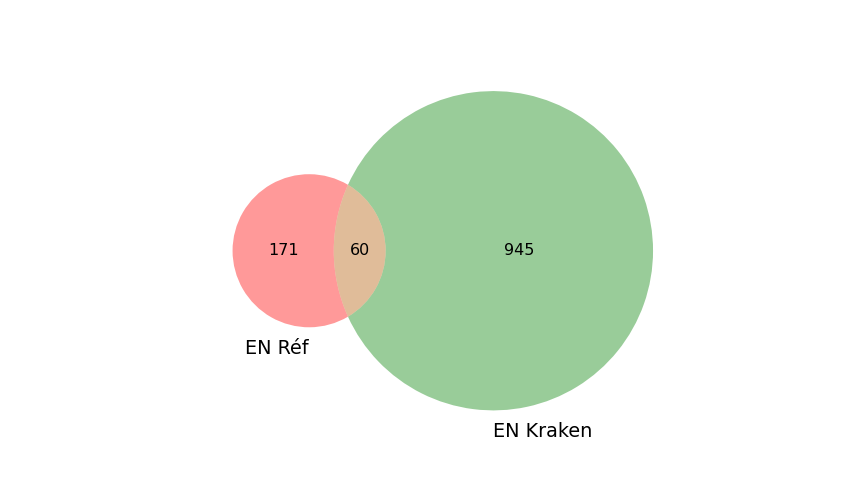
\includegraphics[width=.99\textwidth]{IMAGES/ELTeC_INTERSECTIONS_spaCy3.5.1/CASTRO-OSORIO_quatro-novelas_krakenbase.txt_spacy-lg-concat.json_intersection.png}
%    \caption{Kraken-\textsc{spaCy\_lg}}
 
%   \label{fig: }
%   \end{subfigure}
%   \end{minipage}
%   %%
% %\caption{}
% %\label{fig:INTERSECTION_NOAILLES}
% %% [heigH=4cm] enlevé--> passe mal sur ACM
%   \begin{minipage}{7cm}
%   \begin{subfigure}{0.99\textwidth}
%   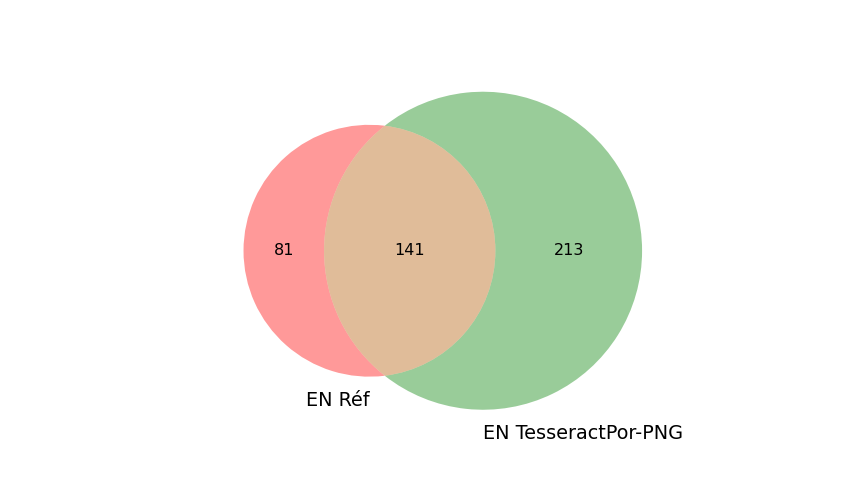
\includegraphics[width=.99\textwidth]{IMAGES/ELTeC_INTERSECTIONS_spaCy3.5.1/CASTRO-OSORIO_quatro-novelas_TesseractPor-PNG.txt_spacy-sm-concat.json_intersection.png} 
%   \caption{Tesseract-\textsc{spacy\_sm}}
%   \label{fig:}
%   \end{subfigure}
%     \end{minipage}
%   %
%   \begin{minipage}{7cm}
%   \begin{subfigure}{0.99\textwidth}
%   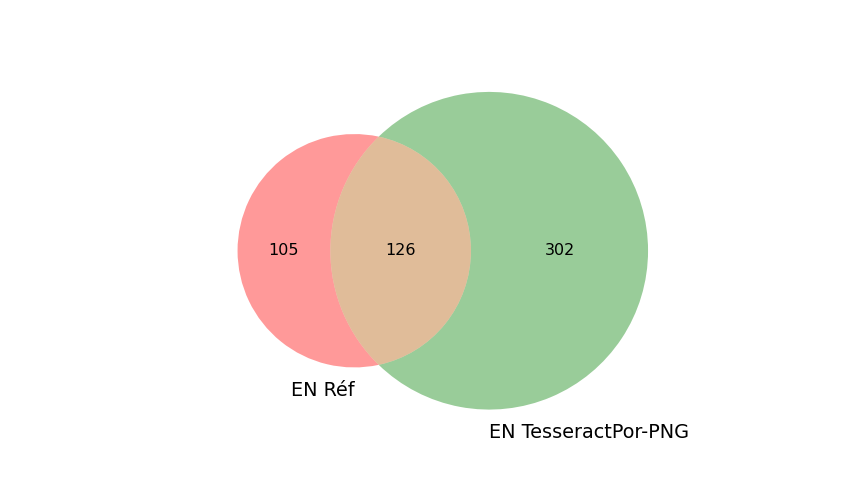
\includegraphics[width=.99\textwidth]{IMAGES/ELTeC_INTERSECTIONS_spaCy3.5.1/CASTRO-OSORIO_quatro-novelas_TesseractPor-PNG.txt_spacy-lg-concat.json_intersection.png}
%    \caption{Tesseract-\textsc{spaCy\_lg}}
%   \label{fig: }
%   \end{subfigure}
%   \end{minipage}
% \caption{Intersections entre les EN (spaCy\_lg, stanza) issues des textes de référence et des versions OCR (Kraken et Tesseract) -- Anna Castro-Osorio, \textit{Quattro Novelas}.}
% \label{fig:}
% \end{figure}

%____DE QUEIROZ
% \begin{figure}
% \begin{minipage}{7cm}
%   \begin{subfigure}{0.99\textwidth}
%   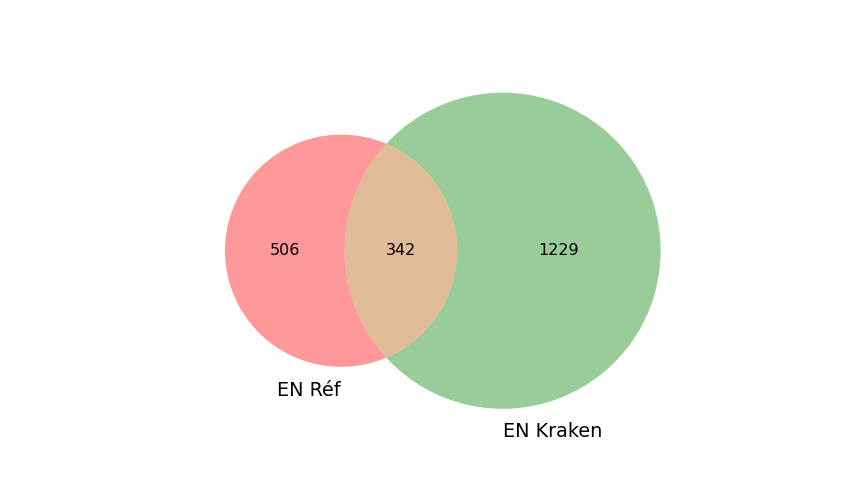
\includegraphics[width=.99\textwidth]{IMAGES/ELTeC_INTERSECTIONS_spaCy3.5.1/DE-QUEIROS_o-crime-do-padre-ama_krakenbase.txt_spacy-sm-concat.json_intersection.png} 
%   \caption{Kraken-\textsc{spaCy\_sm}}
%   \label{fig:TROLLOP_DIST_KRAKENBASE_LG}
%   \end{subfigure}
%   \end{minipage}
%   %
%   \begin{minipage}{7cm}
%   \begin{subfigure}{0.99\textwidth}
%   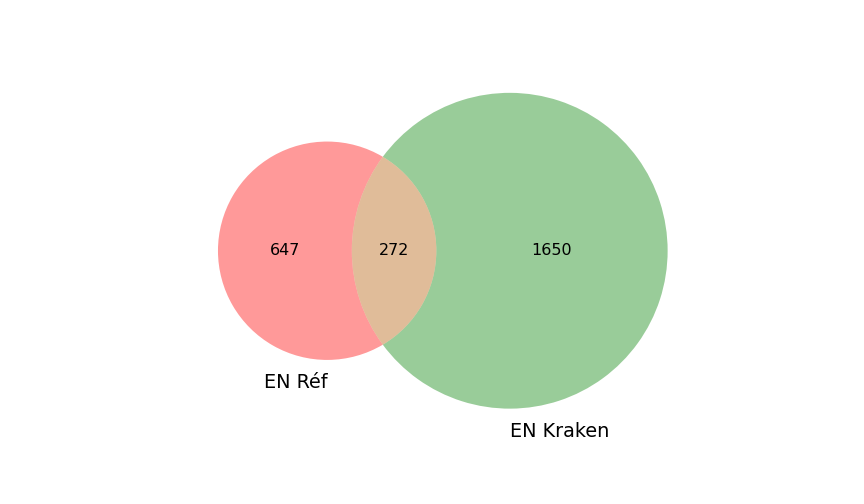
\includegraphics[width=.99\textwidth]{IMAGES/ELTeC_INTERSECTIONS_spaCy3.5.1/DE-QUEIROS_o-crime-do-padre-ama_krakenbase.txt_spacy-lg-concat.json_intersection.png}
%    \caption{Kraken-\textsc{spaCy\_lg}}
 
%   \label{fig: }
%   \end{subfigure}
%   \end{minipage}
%   %%
% %\caption{}
% %\label{fig:INTERSECTION_NOAILLES}
% %% [heigH=4cm] enlevé--> passe mal sur ACM
%   \begin{minipage}{7cm}
%   \begin{subfigure}{0.99\textwidth}
%   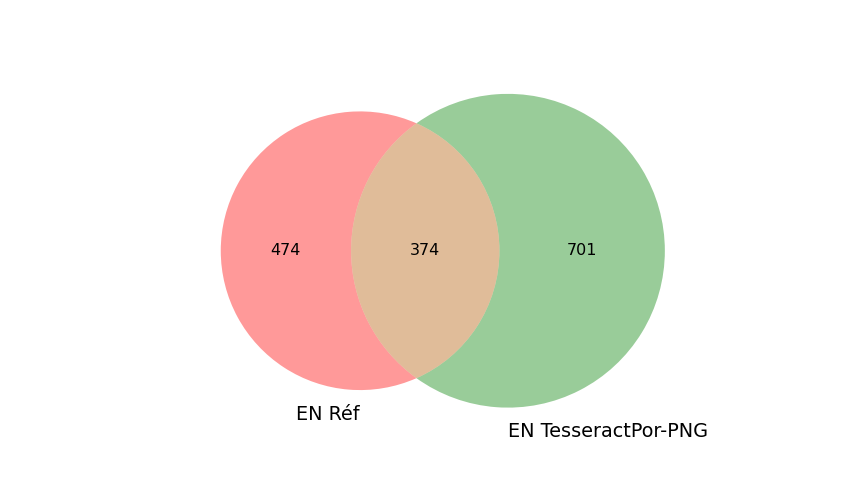
\includegraphics[width=.99\textwidth]{IMAGES/ELTeC_INTERSECTIONS_spaCy3.5.1/DE-QUEIROS_o-crime-do-padre-ama_TesseractPor-PNG.txt_spacy-sm-concat.json_intersection.png} 
%   \caption{Tesseract-\textsc{spacy\_sm}}
%   \label{fig:}
%   \end{subfigure}
%     \end{minipage}
%   %
%   \begin{minipage}{7cm}
%   \begin{subfigure}{0.99\textwidth}
%   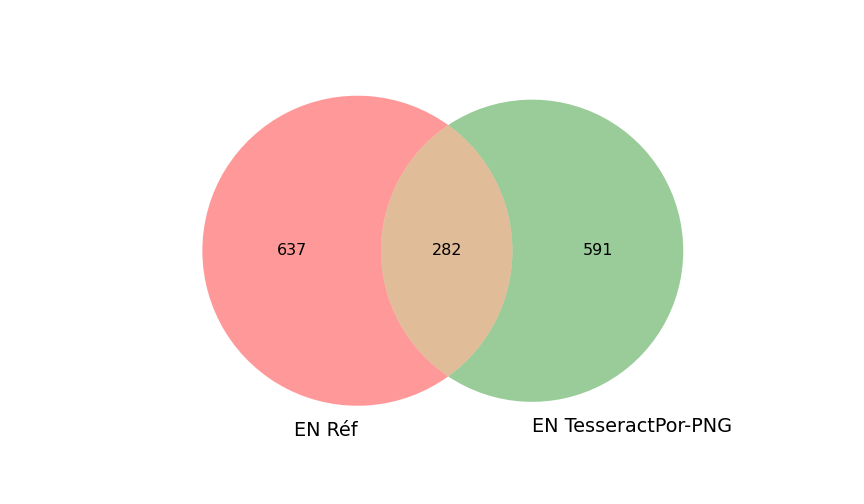
\includegraphics[width=.99\textwidth]{IMAGES/ELTeC_INTERSECTIONS_spaCy3.5.1/DE-QUEIROS_o-crime-do-padre-ama_TesseractPor-PNG.txt_spacy-lg-concat.json_intersection.png}
%    \caption{Tesseract-\textsc{spaCy\_lg}}
%   \label{fig: }
%   \end{subfigure}
%   \end{minipage}
% \caption{Intersections entre les EN (\texttt{spaCy\_sm, spacy\_lg}) issues des textes de référence et des versions OCR (Kraken et Tesseract) -- Eça de Queiroz, \textit{O crime do padre amoro, Cenas da vida devota} ; exemple d'un mauvais OCR, corpus ELTeC portugais.}
% \label{fig:}
% \end{figure}

%_____INTERSECTIONS EN vs. EN corrigées (spacy_lg)


%____BRONTË
% \begin{figure}
% \begin{minipage}{9cm}
%   \begin{subfigure}{1\textwidth}
%   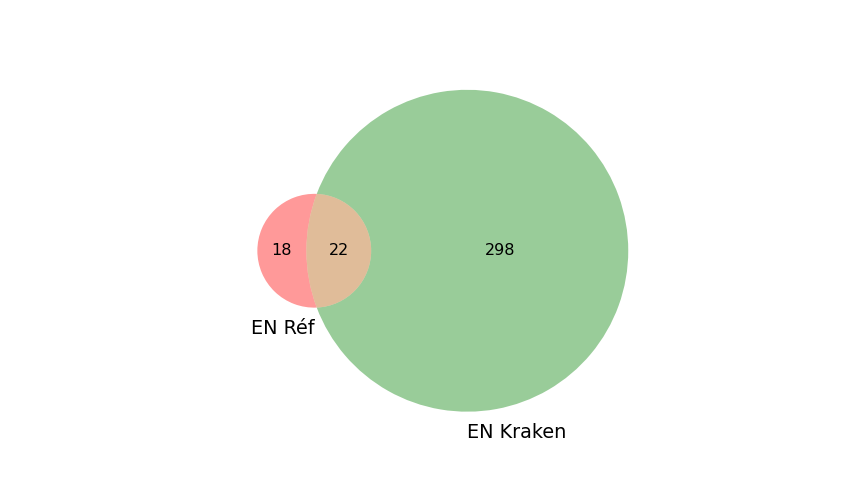
\includegraphics[width=1\textwidth]{IMAGES/ELTeC_INTERSECTIONS_spaCy3.5.1/BRONTE_Wuthering-heights_Kraken.txt_spacy-lg-concat.json_intersection.png} 
%   \caption{Kraken-\textsc{spaCy\_lg}}
%   \label{fig:TROLLOP_DIST_KRAKENBASE_LG}
%   \end{subfigure}
%   \end{minipage}
%   %
%   \begin{minipage}{9cm}
%   \begin{subfigure}{1\textwidth}
%   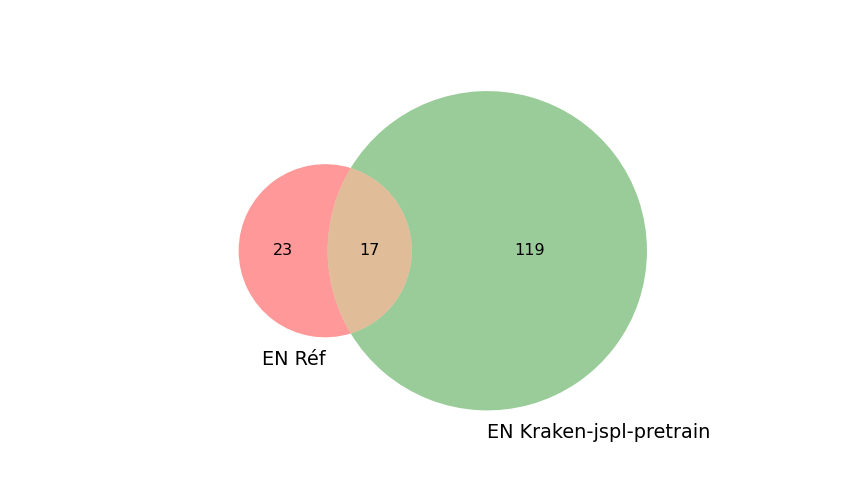
\includegraphics[width=1\textwidth]{IMAGES/ELTeC_INTERSECTIONS_spaCy3.5.1/BRONTE_Wuthering-heights_Kraken_jamspell-cor.txt_spacy-lg-concat.json_intersection.png}
%    \caption{Kraken-JamSpell pré-entraîné-\textsc{spaCy\_lg}}
 
%   \label{fig: }
%   \end{subfigure}
%   \end{minipage}
%   %%
% %\caption{}
% %\label{fig:INTERSECTION_NOAILLES}
% %% [heigH=4cm] enlevé--> passe mal sur ACM
%   \begin{minipage}{9cm}
%   \begin{subfigure}{1\textwidth}
%   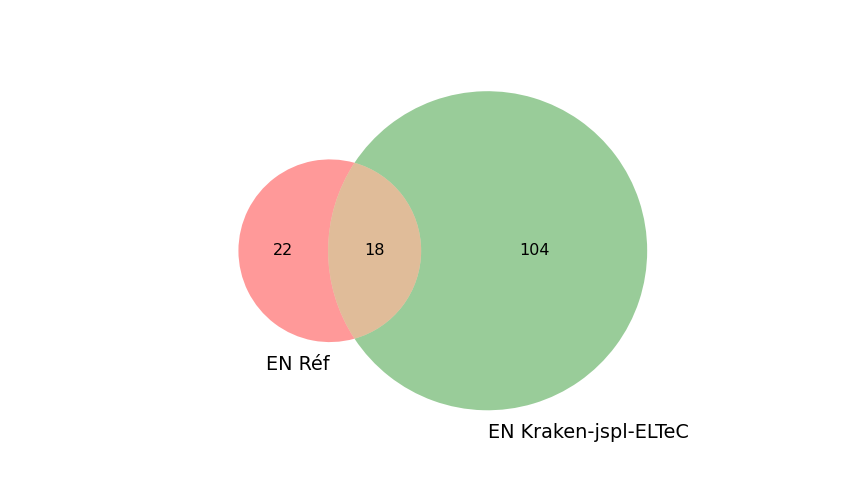
\includegraphics[width=1\textwidth]{IMAGES/ELTeC_INTERSECTIONS_spaCy3.5.1/BRONTE_Wuthering-heights_Kraken_jamspell-ELTeCmodel-en.txt_spacy-lg-concat.json_intersection.png} 
%   \caption{Kraken-JamSpell-ELTeC-\textsc{spacy\_lg}}
%   \label{fig:}
%   \end{subfigure}
%     \end{minipage}
% \caption{Intersections entre les EN (spaCy\_lg) issues des versions OCR (Kraken) et celles corrigées avec JamSpell (modèle pré-entraîné et modèle ELTeC) -- Emily Brontë, \textit{Wuthering HeigHs}.}
% \label{fig:}
% \end{figure}

%____REYNOLDS
% \begin{figure}
% \begin{minipage}{7cm}
%   \begin{subfigure}{1\textwidth}
%   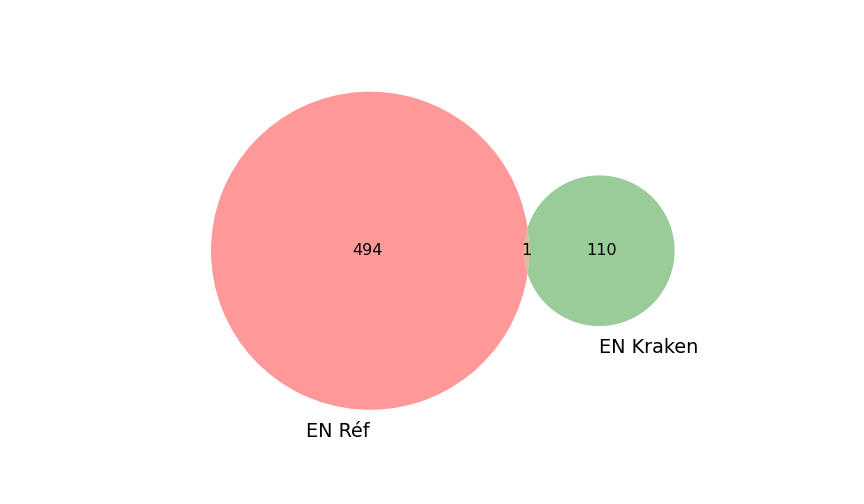
\includegraphics[width=1\textwidth]{IMAGES/ELTeC_INTERSECTIONS_spaCy3.5.1/REYNOLDS_The-Mysteries-of-London_Kraken.txt_spacy-lg-concat.json_intersection.png} 
%   \caption{Kraken-\textsc{spaCy\_lg}}
%   \label{fig:TROLLOP_DIST_KRAKENBASE_LG}
%   \end{subfigure}
%   \end{minipage}
%   %
%   \begin{minipage}{7cm}
%   \begin{subfigure}{1\textwidth}
%   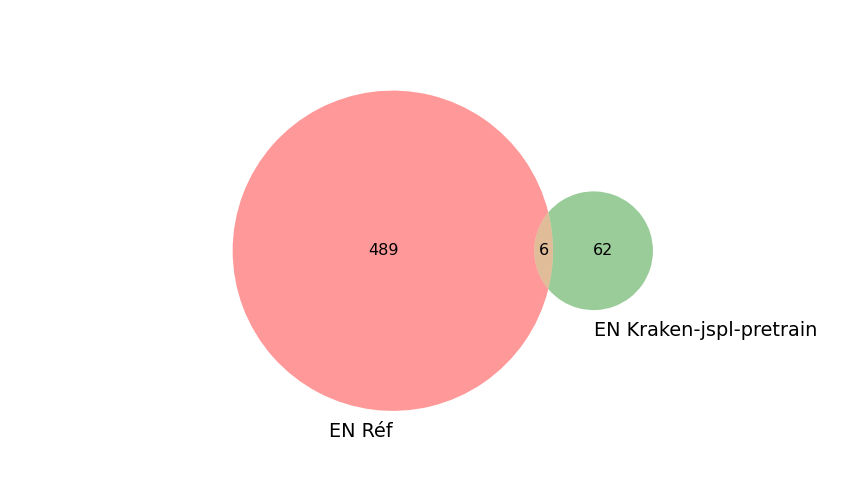
\includegraphics[width=1\textwidth]{IMAGES/ELTeC_INTERSECTIONS_spaCy3.5.1/REYNOLDS_The-Mysteries-of-London_Kraken_jamspell-cor.txt_spacy-lg-concat.json_intersection.png}
%    \caption{Kraken-JamSpell pré-entraîné-\textsc{spaCy\_lg}}
 
%   \label{fig: }
%   \end{subfigure}
%   \end{minipage}
%   %%
% %\caption{}
% %\label{fig:INTERSECTION_NOAILLES}
% %% [heigH=4cm] enlevé--> passe mal sur ACM
%   \begin{minipage}{7cm}
%   \begin{subfigure}{1\textwidth}
%   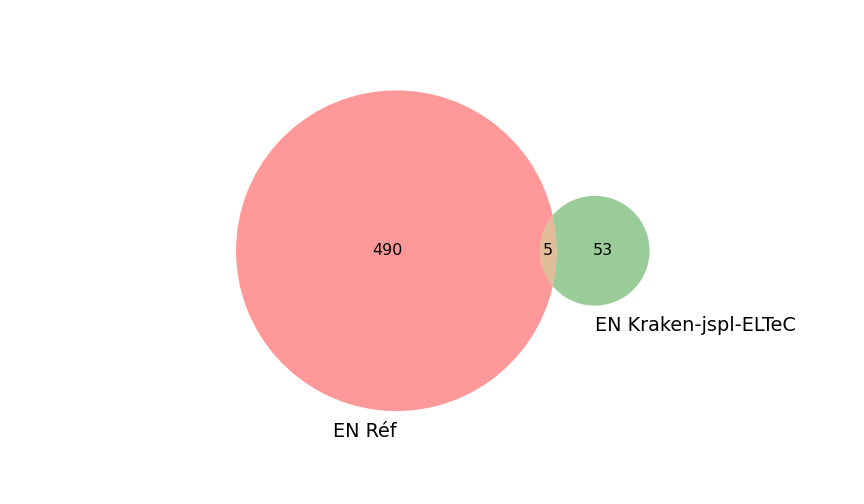
\includegraphics[width=1\textwidth]{IMAGES/ELTeC_INTERSECTIONS_spaCy3.5.1/REYNOLDS_The-Mysteries-of-London_Kraken_jamspell-ELTeCmodel-en.txt_spacy-lg-concat.json_intersection.png} 
%   \caption{Kraken-JamSpell-ELTeC-\textsc{spacy\_lg}}
%   \label{fig:}
%   \end{subfigure}
%     \end{minipage}
% \caption{Intersections entre les EN (spaCy\_lg) issues des versions OCR (Kraken) et celles corrigées avec JamSpell (modèle pré-entraîné et modèle ELTeC) -- G. W. M. Reynolds, \textit{The Mysteries of London}.}
% \label{fig:}
% \end{figure}

%____MAUPASSANT
% \begin{figure}
% \begin{minipage}{9cm}
%   \begin{subfigure}{1\textwidth}
%   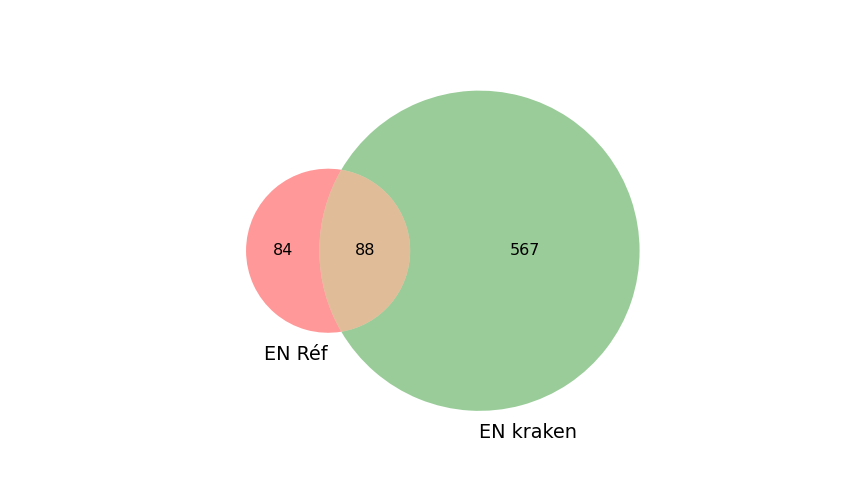
\includegraphics[width=1\textwidth]{IMAGES/ELTeC_INTERSECTIONS_spaCy3.5.1/MAUPASSANT_une-vie_Kraken-base.txt_spacy-lg-concat.json_intersection.png} 
%   \caption{Kraken-\textsc{spaCy\_lg}}
%   \label{fig:TROLLOP_DIST_KRAKENBASE_LG}
%   \end{subfigure}
%   \end{minipage}
%   %
%   \begin{minipage}{9cm}
%   \begin{subfigure}{1\textwidth}
%   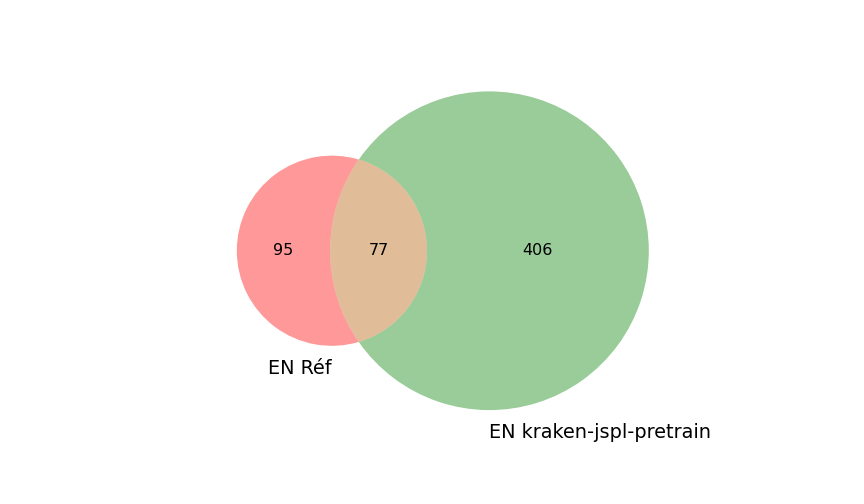
\includegraphics[width=1\textwidth]{IMAGES/ELTeC_INTERSECTIONS_spaCy3.5.1/MAUPASSANT_une-vie_Kraken-base_jamspell-pretrain-fr.txt_spacy-lg-concat.json_intersection.png}
%    \caption{Kraken-JamSpell pré-entraîné-\textsc{spaCy\_lg}}
 
%   \label{fig: }
%   \end{subfigure}
%   \end{minipage}
%   %%
% %\caption{}
% %\label{fig:INTERSECTION_NOAILLES}
% %% [heigH=4cm] enlevé--> passe mal sur ACM
%   \begin{minipage}{9cm}
%   \begin{subfigure}{1\textwidth}
%   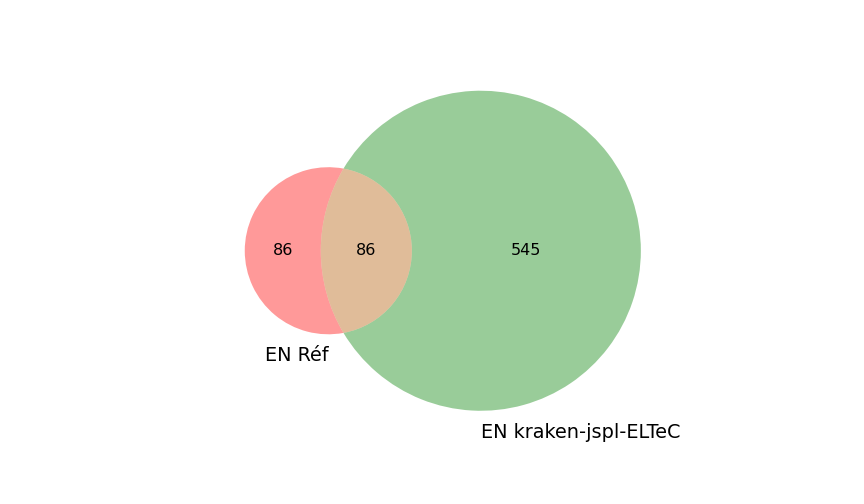
\includegraphics[width=1\textwidth]{IMAGES/ELTeC_INTERSECTIONS_spaCy3.5.1/MAUPASSANT_une-vie_Kraken-base_jamspell-ELTeCmodel-fr.txt_spacy-lg-concat.json_intersection.png} 
%   \caption{Kraken-JamSpell-ELTeC-\textsc{spacy\_lg}}
%   \label{fig:}
%   \end{subfigure}
%     \end{minipage}
% \caption{Intersections entre les EN (spaCy\_lg) issues des versions OCR (Kraken) et celles corrigées avec JamSpell (modèle pré-entraîné et modèle ELTeC) -- Guy de Maupassant, \textit{Une vie}.}
% \label{fig:}
% \end{figure}

%____DAUDET
% \begin{figure}
% \begin{minipage}{7cm}
%   \begin{subfigure}{1\textwidth}
%   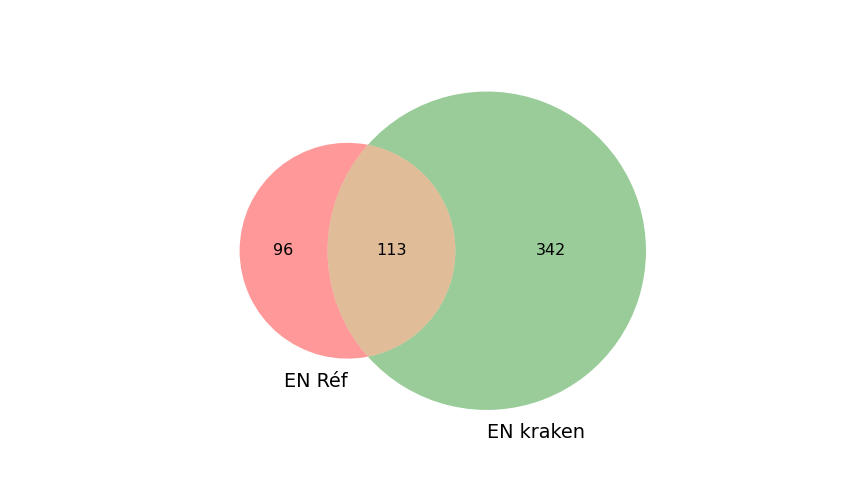
\includegraphics[width=1\textwidth]{IMAGES/ELTeC_INTERSECTIONS_spaCy3.5.1/DAUDET_petit-chose_Kraken-base.txt_spacy-lg-concat.json_intersection.png} 
%   \caption{Kraken-\textsc{spaCy\_lg}}
%   \label{fig:TROLLOP_DIST_KRAKENBASE_LG}
%   \end{subfigure}
%   \end{minipage}
%   %
%   \begin{minipage}{7cm}
%   \begin{subfigure}{1\textwidth}
%   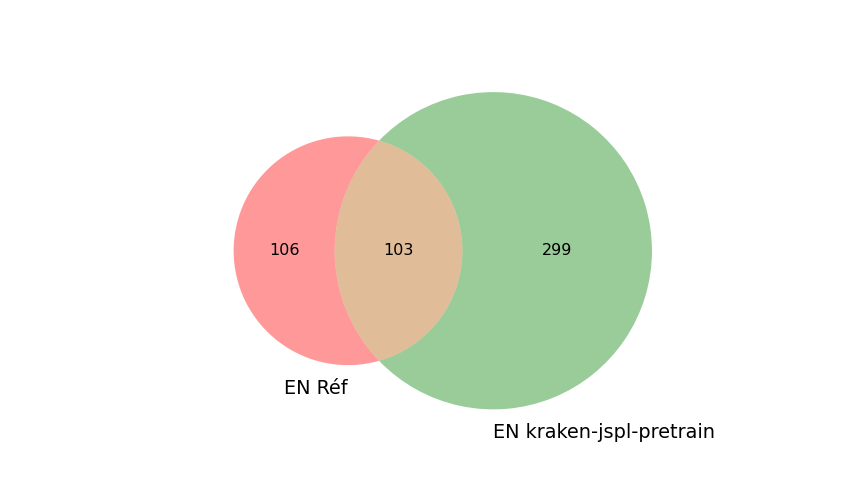
\includegraphics[width=1\textwidth]{IMAGES/ELTeC_INTERSECTIONS_spaCy3.5.1/DAUDET_petit-chose_Kraken-base_jamspell-pretrain-fr.txt_spacy-lg-concat.json_intersection.png}
%    \caption{Kraken-JamSpell pré-entraîné-\textsc{spaCy\_lg}}
 
%   \label{fig: }
%   \end{subfigure}
%   \end{minipage}
%   %%
% %\caption{}
% %\label{fig:INTERSECTION_NOAILLES}
% %% [heigH=4cm] enlevé--> passe mal sur ACM
%   \begin{minipage}{7cm}
%   \begin{subfigure}{1\textwidth}
%   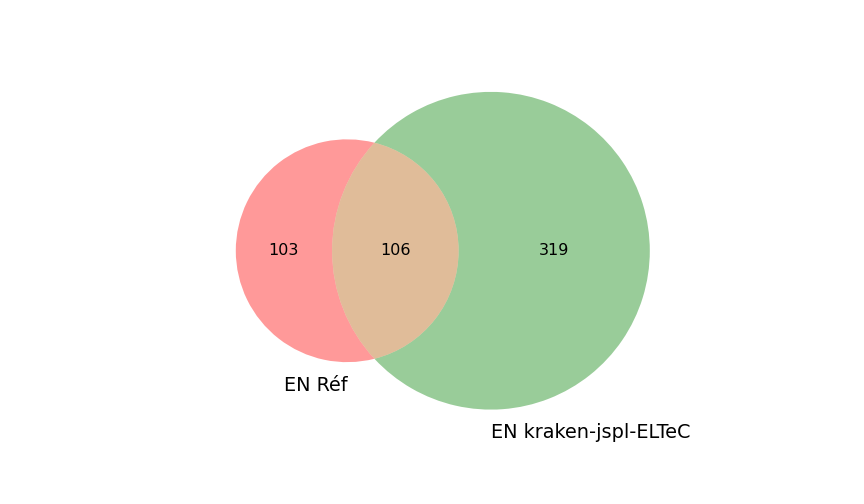
\includegraphics[width=1\textwidth]{IMAGES/ELTeC_INTERSECTIONS_spaCy3.5.1/DAUDET_petit-chose_Kraken-base_jamspell-ELTeCmodel-fr.txt_spacy-lg-concat.json_intersection.png} 
%   \caption{Kraken-JamSpell-ELTeC-\textsc{spacy\_lg}}
%   \label{fig:}
%   \end{subfigure}
%     \end{minipage}
% \caption{Intersections entre les EN (spaCy\_lg) issues des versions OCR (Kraken) et celles corrigées avec JamSpell (modèle pré-entraîné et modèle ELTeC) -- Alphonse Daudet, \textit{Le petit chose}.}
% \label{fig:}
% \end{figure}



%____CASTRO-OSORIO
% \begin{figure}
% \begin{minipage}{9cm}
%   \begin{subfigure}{1\textwidth}
%   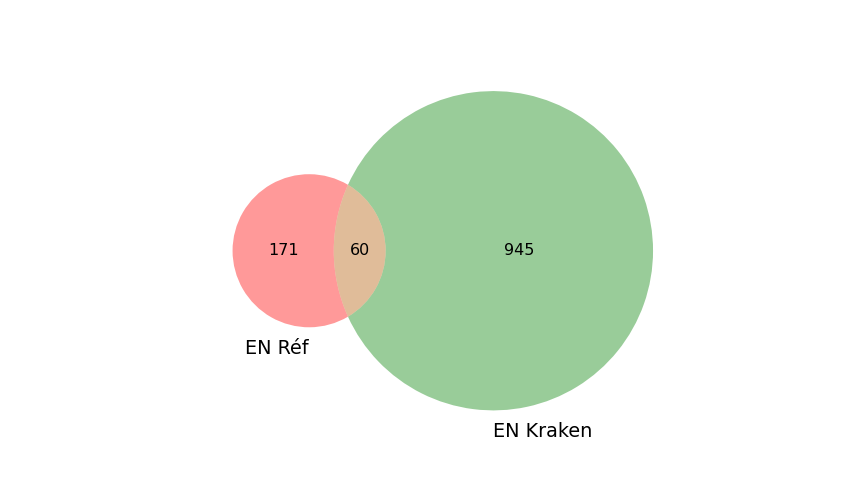
\includegraphics[width=1\textwidth]{IMAGES/ELTeC_INTERSECTIONS_spaCy3.5.1/CASTRO-OSORIO_quatro-novelas_krakenbase.txt_spacy-lg-concat.json_intersection.png} 
%   \caption{Kraken-\textsc{spaCy\_lg}}
%   \label{fig:TROLLOP_DIST_KRAKENBASE_LG}
%   \end{subfigure}
%   \end{minipage}
%   %
%   \begin{minipage}{9cm}
%   \begin{subfigure}{1\textwidth}
%   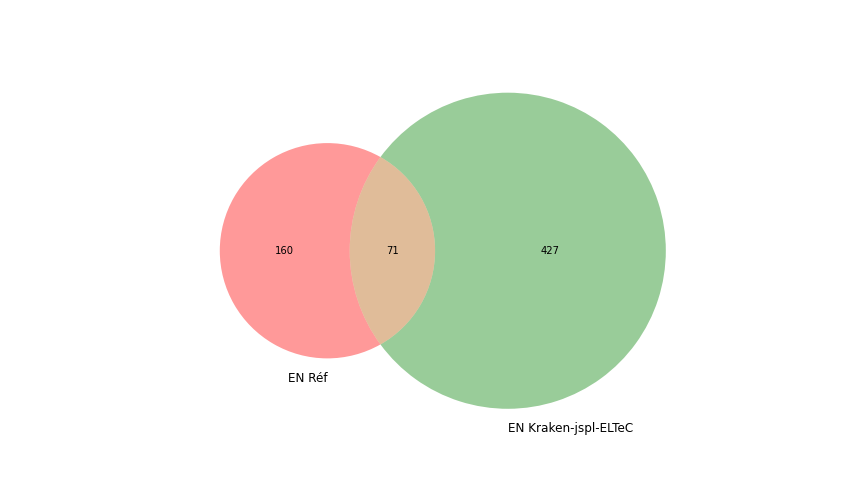
\includegraphics[width=1\textwidth]{IMAGES/ELTeC_INTERSECTIONS_spaCy3.5.1/CASTRO-OSORIO_quatro-novelas_krakenbase_jamspell-ELTeCmodel-por.txt_spacy-lg-concat.json_intersection.png}
%   \caption{Kraken-JamSpell-ELTeC-\textsc{spacy\_lg}}
%   \label{fig:}
%   \end{subfigure}
%     \end{minipage}
% \caption{Intersections entre les EN (spaCy\_lg) issues des versions OCR (Kraken) et celles corrigées avec JamSpell (modèle ELTeC) -- Anna Castro-Osorio, \textit{Quattro Novelas}.}
% \label{fig:}
% \end{figure}

%____DE QUEIROZ
% \begin{figure}
% \begin{minipage}{7cm}
%   \begin{subfigure}{1\textwidth}
%   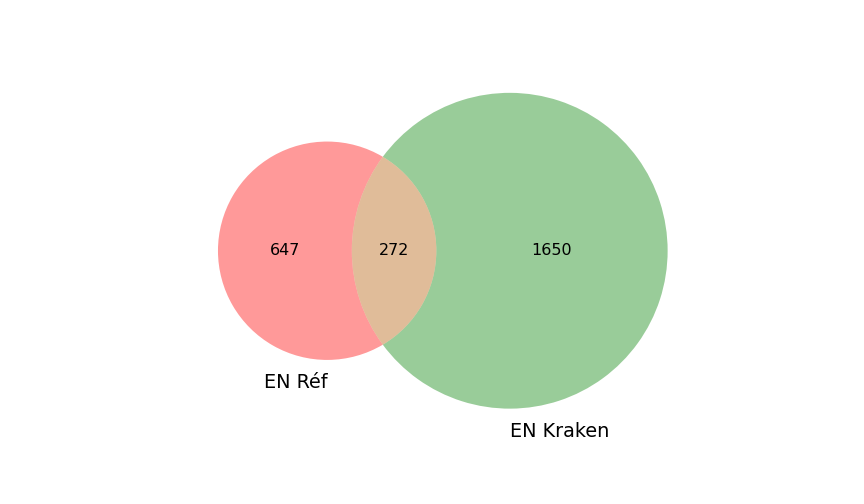
\includegraphics[width=1\textwidth]{IMAGES/ELTeC_INTERSECTIONS_spaCy3.5.1/DE-QUEIROS_o-crime-do-padre-ama_krakenbase.txt_spacy-lg-concat.json_intersection.png} 
%   \caption{Kraken-\textsc{spaCy\_lg}}
%   \label{fig:TROLLOP_DIST_KRAKENBASE_LG}
%   \end{subfigure}
%   \end{minipage}
%   %
%   \begin{minipage}{7cm}
%   \begin{subfigure}{1\textwidth}
%   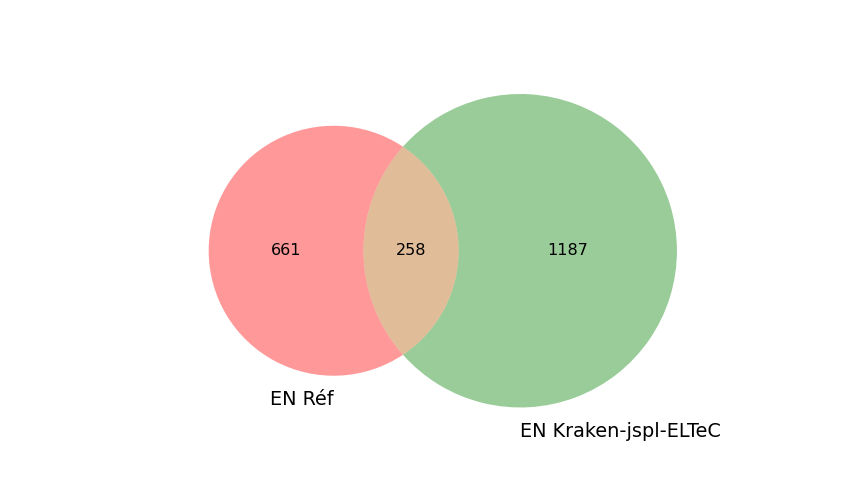
\includegraphics[width=1\textwidth]{IMAGES/ELTeC_INTERSECTIONS_spaCy3.5.1/DE-QUEIROS_o-crime-do-padre-ama_krakenbase_jamspell-ELTeCmodel-por.txt_spacy-lg-concat.json_intersection.png}
%   \caption{Kraken-JamSpell-ELTeC-\textsc{spacy\_lg}}
%   \label{fig:}
%   \end{subfigure}
%     \end{minipage}
% \caption{Intersections entre les EN (spaCy\_lg) issues des versions OCR (Kraken) et celles corrigées avec JamSpell (modèle ELTeC) -- Eça de Queiroz, \textit{O crime do padre amoro, Cenas da vida devota}.}
% \label{fig:}
% \end{figure}

%_____INTERSECTIONS EN vs. EN corrigées (stanza)
%____TROLLOPPE
% \begin{figure}
% \begin{minipage}{9cm}
%   \begin{subfigure}{1\textwidth}
%   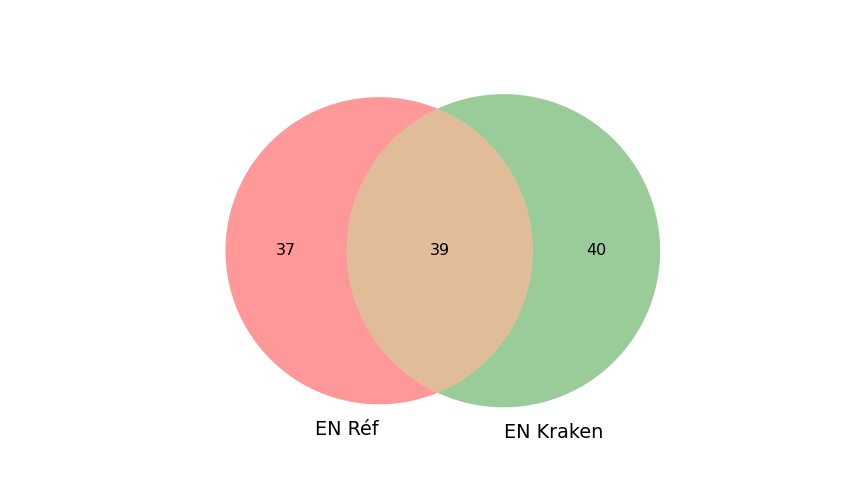
\includegraphics[width=1\textwidth]{IMAGES/ELTeC_INTERSECTIONS_stanza/TROLLOPE_Adventure_Kraken.txt_stanza-concat.json_intersection.png} 
%   \caption{Kraken-\textsc{Stanza}}
%   \label{fig:TROLLOP_DIST_KRAKENBASE_LG}
%   \end{subfigure}
%   \end{minipage}
%   %
%   \begin{minipage}{9cm}
%   \begin{subfigure}{1\textwidth}
%   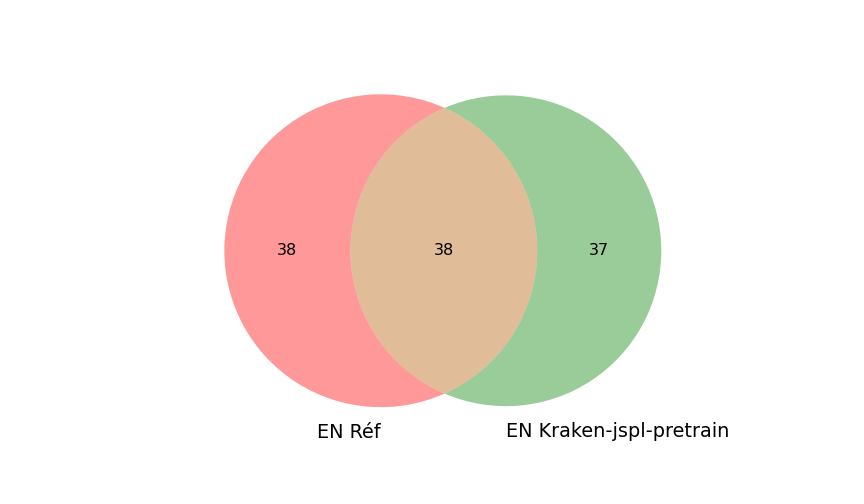
\includegraphics[width=1\textwidth]{IMAGES/ELTeC_INTERSECTIONS_stanza/TROLLOPE_Adventure_Kraken_jamspell-cor.txt_stanza-concat.json_intersection.png}
%    \caption{Kraken-JamSpell pré-entraîné-\textsc{Stanza}}
 
%   \label{fig: }
%   \end{subfigure}
%   \end{minipage}
%   %%
% %\caption{}
% %\label{fig:INTERSECTION_NOAILLES}
% %% [heigH=4cm] enlevé--> passe mal sur ACM
%   \begin{minipage}{9cm}
%   \begin{subfigure}{1\textwidth}
%   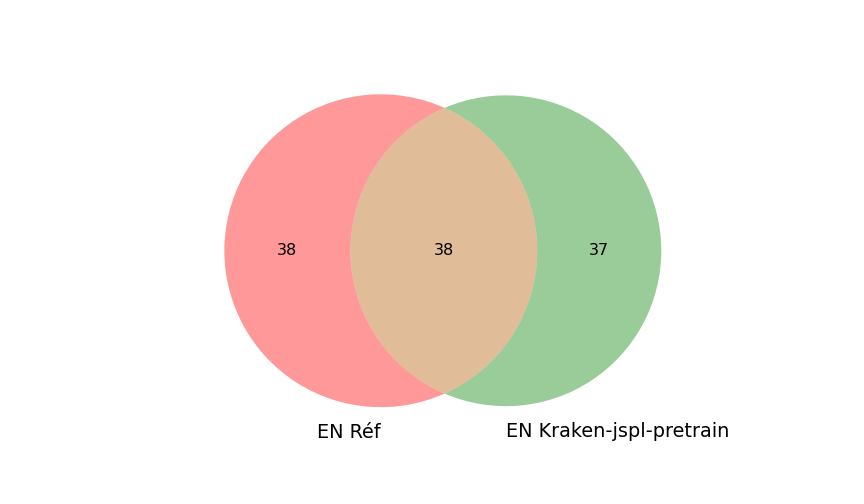
\includegraphics[width=1\textwidth]{IMAGES/ELTeC_INTERSECTIONS_stanza/TROLLOPE_Adventure_Kraken_jamspell-cor.txt_stanza-concat.json_intersection.png} 
%   \caption{Kraken-JamSpell-ELTeC-\textsc{Stanza}}
%   \label{fig:}
%   \end{subfigure}
%     \end{minipage}
% \caption{Intersections entre les EN (Stanza) issues des versions OCR (Kraken) et celles corrigées avec JamSpell (modèle pré-entraîné et modèle ELTeC) -- Frances Trolloppe, \textit{The Life and Adventures of M. Armstrong}.}
% \label{fig:}
% \end{figure}

% %____BRONTË
% \begin{figure}
% \begin{minipage}{9cm}
%   \begin{subfigure}{1\textwidth}
%   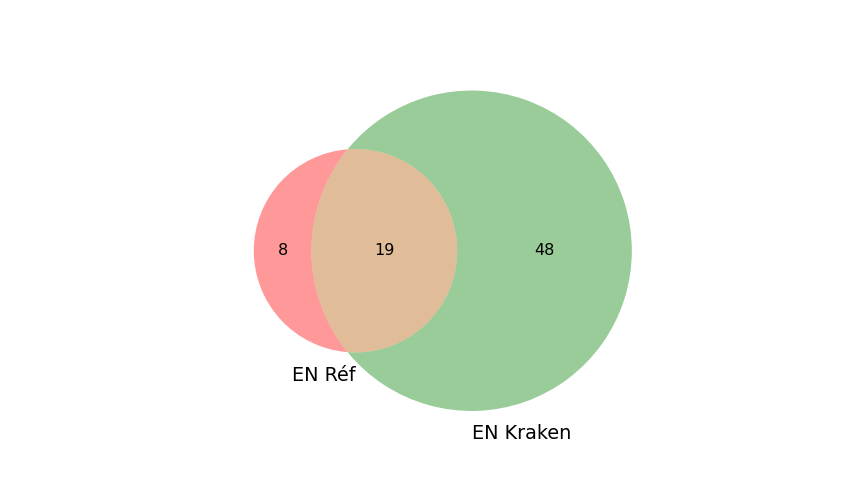
\includegraphics[width=1\textwidth]{IMAGES/ELTeC_INTERSECTIONS_stanza/BRONTE_Wuthering-heights_Kraken.txt_stanza-concat.json_intersection.png} 
%   \caption{Kraken-\textsc{Stanza}}
%   \label{fig:TROLLOP_DIST_KRAKENBASE_LG}
%   \end{subfigure}
%   \end{minipage}
%   %
%   \begin{minipage}{9cm}
%   \begin{subfigure}{1\textwidth}
%   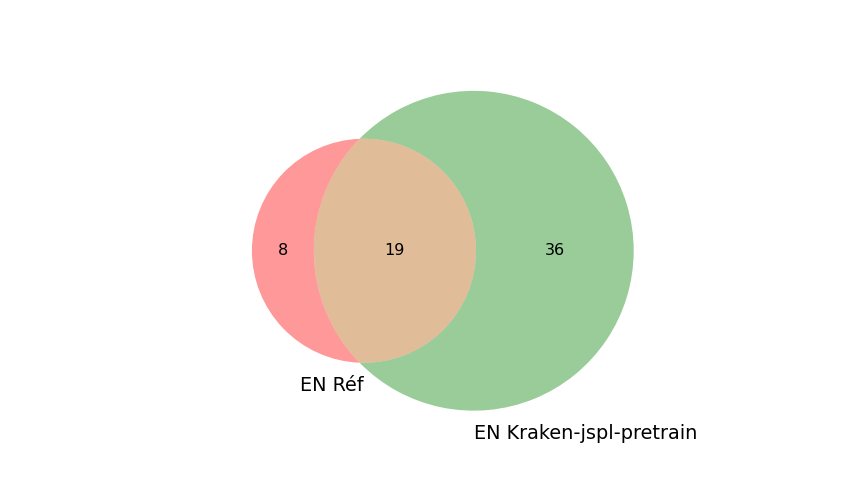
\includegraphics[width=1\textwidth]{IMAGES/ELTeC_INTERSECTIONS_stanza/BRONTE_Wuthering-heights_Kraken_jamspell-cor.txt_stanza-concat.json_intersection.png}
%    \caption{Kraken-JamSpell pré-entraîné-\textsc{Stanza}}
 
%   \label{fig: }
%   \end{subfigure}
%   \end{minipage}
%   %%
% %\caption{}
% %\label{fig:INTERSECTION_NOAILLES}
% %% [heigH=4cm] enlevé--> passe mal sur ACM
%   \begin{minipage}{9cm}
%   \begin{subfigure}{1\textwidth}
%   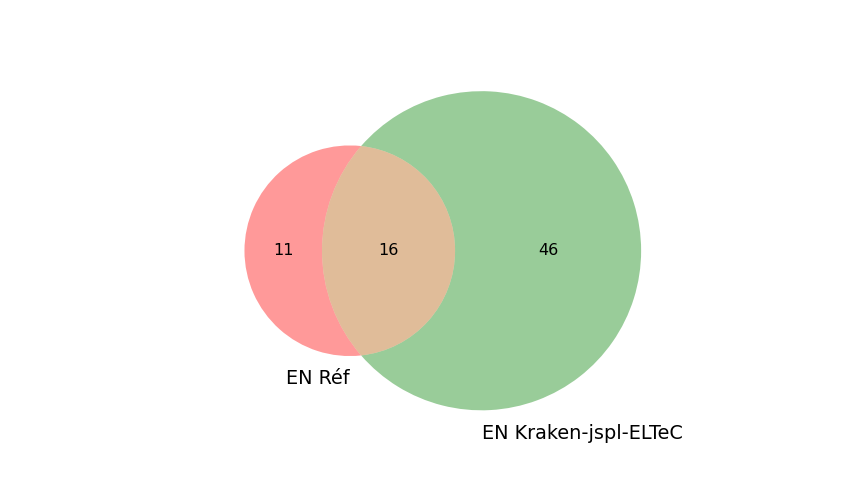
\includegraphics[width=1\textwidth]{IMAGES/ELTeC_INTERSECTIONS_stanza/BRONTE_Wuthering-heights_Kraken_jamspell-ELTeCmodel-en.txt_stanza-concat.json_intersection.png} 
%   \caption{Kraken-JamSpell-ELTeC-\textsc{Stanza}}
%   \label{fig:}
%   \end{subfigure}
%     \end{minipage}
% \caption{Intersections entre les EN (Stanza) issues des versions OCR (Kraken) et celles corrigées avec JamSpell (modèle pré-entraîné et modèle ELTeC) -- Emily Brontë, \textit{Wuthering HeigHs}.}
% \label{fig:}
% \end{figure}

% %____REYNOLDS

% %____MAUPASSANT

% %____DAUDET

% %____ADAM

% %____DINIZ

% %____CASTRO-OSORIO

% %____DE QUEIROZ


%_____INTERSECTIONS-jspl (extra)
% DÉCOMMENTER SI BESOIN !!!!
%____TROLLOPPE
% \begin{figure}
% \begin{minipage}{7cm}
%   \begin{subfigure}{0.99\textwidth}
%   \includegraphics[width=.99\textwidth]{IMAGES/ELTeC_INTERSECTIONS_spaCy3.5.1/TROLLOPE_Adventure_Kraken_jamspell-cor.txt_spacy-lg-concat.json_intersection.png} 
%   \caption{Kraken-JamSpell pré-entraîné-\textsc{spaCy\_lg}}
%   \label{fig:TROLLOP_DIST_KRAKENBASE_LG}
%   \end{subfigure}
%   \end{minipage}
%   %
%   \begin{minipage}{7cm}
%   \begin{subfigure}{0.99\textwidth}
%   \includegraphics[width=.99\textwidth]{IMAGES/ELTeC_INTERSECTIONS_stanza/TROLLOPE_Adventure_Kraken_jamspell-cor.txt_stanza-concat.json_intersection.png}
%    \caption{Kraken-JamSpell pré-entraîné-\textsc{Stanza}}
 
%   \label{fig: }
%   \end{subfigure}
%   \end{minipage}
%   %%
% %\caption{}
% %\label{fig:INTERSECTION_NOAILLES}
% %% [heigH=4cm] enlevé--> passe mal sur ACM
%   \begin{minipage}{7cm}
%   \begin{subfigure}{0.99\textwidth}
%   \includegraphics[width=.99\textwidth]{IMAGES/ELTeC_INTERSECTIONS_spaCy3.5.1/TROLLOPE_Adventure_Tesseract-PNG_jamspell-cor.txt_spacy-lg-concat.json_intersection.png} 
%   \caption{Tesseract-JamSpell pré-entraîné-\textsc{spacy\_lg}}
%   \label{fig:}
%   \end{subfigure}
%     \end{minipage}
%   %
%   \begin{minipage}{7cm}
%   \begin{subfigure}{0.99\textwidth}
%   \includegraphics[width=.99\textwidth]{IMAGES/ELTeC_INTERSECTIONS_stanza/TROLLOPE_Adventure_Tesseract-PNG_jamspell-cor.txt_stanza-concat.json_intersection.png}
%    \caption{Tesseract-JamSpell pré-entraîné-\textsc{stanza}}
%   \label{fig: }
%   \end{subfigure}
%   \end{minipage}
% \caption{Intersections entre les EN (spaCy\_lg, stanza) issues des textes de référence et des versions OCR (Kraken et Tesseract) corrigées avec JamSpell -- Frances Trolloppe, \textit{The Life and Adventures of M. Armstrong}.}
% \label{fig:}
% \end{figure}

% %____BRONTË
% \begin{figure}
% \begin{minipage}{7cm}
%   \begin{subfigure}{0.99\textwidth}
%   \includegraphics[width=.99\textwidth]{IMAGES/ELTeC_INTERSECTIONS_spaCy3.5.1/BRONTE_Wuthering-heigHs_Kraken_jamspell-cor.txt_spacy-lg-concat.json_intersection.png} 
%   \caption{Kraken-JamSpell pré-entraîné-\textsc{spaCy\_lg}}
%   \label{fig:TROLLOP_DIST_KRAKENBASE_LG}
%   \end{subfigure}
%   \end{minipage}
%   %
%   \begin{minipage}{7cm}
%   \begin{subfigure}{0.99\textwidth}
%   \includegraphics[width=.99\textwidth]{IMAGES/ELTeC_INTERSECTIONS_stanza/BRONTE_Wuthering-heigHs_Kraken_jamspell-cor.txt_stanza-concat.json_intersection.png}
%    \caption{Kraken-JamSpell pré-entraîné-\textsc{Stanza}}
 
%   \label{fig: }
%   \end{subfigure}
%   \end{minipage}
%   %%
% %\caption{}
% %\label{fig:INTERSECTION_NOAILLES}
% %% [heigH=4cm] enlevé--> passe mal sur ACM
%   \begin{minipage}{7cm}
%   \begin{subfigure}{0.99\textwidth}
%   \includegraphics[width=.99\textwidth]{IMAGES/ELTeC_INTERSECTIONS_spaCy3.5.1/BRONTE_Wuthering-heigHs_Tesseract-PNG_jamspell-cor.txt_spacy-lg-concat.json_intersection.png} 
%   \caption{Tesseract-JamSpell pré-entraîné-\textsc{spacy\_lg}}
%   \label{fig:}
%   \end{subfigure}
%     \end{minipage}
%   %
%   \begin{minipage}{7cm}
%   \begin{subfigure}{0.99\textwidth}
%   \includegraphics[width=.99\textwidth]{IMAGES/ELTeC_INTERSECTIONS_stanza/BRONTE_Wuthering-heigHs_Tesseract-PNG_jamspell-cor.txt_stanza-concat.json_intersection.png}
%    \caption{Tesseract-JamSpell pré-entraîné-\textsc{stanza}}
%   \label{fig: }
%   \end{subfigure}
%   \end{minipage}
% \caption{Intersections entre les EN (spaCy\_lg, stanza) issues des textes de référence et des versions OCR (Kraken et Tesseract) corrigées avec JamSpell -- Emily Brontë, \textit{Wuthering HeigHs}.}
% \label{fig:}
% \end{figure}

% %----REYNOLDS
% \begin{figure}
% \begin{minipage}{7cm}
%   \begin{subfigure}{0.99\textwidth}
%   \includegraphics[width=.99\textwidth]{IMAGES/ELTeC_INTERSECTIONS_spaCy3.5.1/REYNOLDS_The-Mysteries-of-London_Kraken_jamspell-cor.txt_spacy-lg-concat.json_intersection.png} 
%   \caption{Kraken-JamSpell pré-entraîné-\textsc{spaCy\_lg}}
%   \label{fig:TROLLOP_DIST_KRAKENBASE_LG}
%   \end{subfigure}
%   \end{minipage}
%   %
%   \begin{minipage}{7cm}
%   \begin{subfigure}{0.99\textwidth}
%   \includegraphics[width=.99\textwidth]{IMAGES/ELTeC_INTERSECTIONS_stanza/REYNOLDS_The-Mysteries-of-London_Kraken_jamspell-cor.txt_stanza-concat.json_intersection.png}
%    \caption{Kraken-JamSpell pré-entraîné-\textsc{Stanza}}
 
%   \label{fig: }
%   \end{subfigure}
%   \end{minipage}
%   %%
% %\caption{}
% %\label{fig:INTERSECTION_NOAILLES}
% %% [heigH=4cm] enlevé--> passe mal sur ACM
%   \begin{minipage}{7cm}
%   \begin{subfigure}{0.99\textwidth}
%   \includegraphics[width=.99\textwidth]{IMAGES/ELTeC_INTERSECTIONS_spaCy3.5.1/REYNOLDS_The-Mysteries-of-London_Tesseract-PNG_jamspell-cor.txt_spacy-lg-concat.json_intersection.png} 
%   \caption{Tesseract-JamSpell pré-entraîné-\textsc{spacy\_lg}}
%   \label{fig:}
%   \end{subfigure}
%     \end{minipage}
%   %
%   \begin{minipage}{7cm}
%   \begin{subfigure}{0.99\textwidth}
%   \includegraphics[width=.99\textwidth]{IMAGES/ELTeC_INTERSECTIONS_stanza/REYNOLDS_The-Mysteries-of-London_Tesseract-PNG_jamspell-cor.txt_stanza-concat.json_intersection.png}
%    \caption{Tesseract-JamSpell pré-entraîné-\textsc{stanza}}
%   \label{fig: }
%   \end{subfigure}
%   \end{minipage}
% \caption{Intersections entre les EN (spaCy\_lg, stanza) issues des textes de référence et des versions OCR (Kraken et Tesseract) corrigées avec JamSpell -- G. M. W. Reynolds, \textit{The Mysteries of London}.}
% \label{fig:}
% \end{figure}

% %____MAUPASSANT
% \begin{figure}
% \begin{minipage}{7cm}
%   \begin{subfigure}{0.99\textwidth}
%   \includegraphics[width=.99\textwidth]{IMAGES/ELTeC_INTERSECTIONS_spaCy3.5.1/MAUPASSANT_une-vie_Kraken-base_jamspell-pretrain-fr.txt_spacy-lg-concat.json_intersection.png} 
%   \caption{Kraken-JamSpell pré-entraîné-\textsc{spaCy\_lg}}
%   \label{fig:TROLLOP_DIST_KRAKENBASE_LG}
%   \end{subfigure}
%   \end{minipage}
%   %
%   \begin{minipage}{7cm}
%   \begin{subfigure}{0.99\textwidth}
%   \includegraphics[width=.99\textwidth]{IMAGES/ELTeC_INTERSECTIONS_stanza/MAUPASSANT_une-vie_Kraken-base_jamspell-pretrain-fr.txt_stanza-concat.json_intersection.png}
%    \caption{Kraken-JamSpell pré-entraîné-\textsc{Stanza}}
 
%   \label{fig: }
%   \end{subfigure}
%   \end{minipage}
%   %%
% %\caption{}
% %\label{fig:INTERSECTION_NOAILLES}
% %% [heigH=4cm] enlevé--> passe mal sur ACM
%   \begin{minipage}{7cm}
%   \begin{subfigure}{0.99\textwidth}
%   \includegraphics[width=.99\textwidth]{IMAGES/ELTeC_INTERSECTIONS_spaCy3.5.1/MAUPASSANT_une-vie_TesseractFra-PNG_jamspell-pretrain-fr.txt_spacy-lg-concat.json_intersection.png} 
%   \caption{Tesseract-JamSpell pré-entraîné-\textsc{spacy\_lg}}
%   \label{fig:}
%   \end{subfigure}
%     \end{minipage}
%   %
%   \begin{minipage}{7cm}
%   \begin{subfigure}{0.99\textwidth}
%   \includegraphics[width=.99\textwidth]{IMAGES/ELTeC_INTERSECTIONS_stanza/MAUPASSANT_une-vie_TesseractFra-PNG_jamspell-pretrain-fr.txt_stanza-concat.json_intersection.png}
%    \caption{Tesseract-JamSpell pré-entraîné-\textsc{stanza}}
%   \label{fig: }
%   \end{subfigure}
%   \end{minipage}
% \caption{Intersections entre les EN (spaCy\_lg, stanza) issues des textes de référence et des versions OCR (Kraken et Tesseract) corrigées avec JamSpell -- Guy de Maupassant, \textit{Une vie}.}
% \label{fig:}
% \end{figure}

% %____DAUDET
% \begin{figure}
% \begin{minipage}{7cm}
%   \begin{subfigure}{0.99\textwidth}
%   \includegraphics[width=.99\textwidth]{IMAGES/ELTeC_INTERSECTIONS_spaCy3.5.1/DAUDET_petit-chose_Kraken-base_jamspell-pretrain-fr.txt_spacy-lg-concat.json_intersection.png} 
%   \caption{Kraken-JamSpell pré-entraîné-\textsc{spaCy\_lg}}
%   \label{fig:TROLLOP_DIST_KRAKENBASE_LG}
%   \end{subfigure}
%   \end{minipage}
%   %
%   \begin{minipage}{7cm}
%   \begin{subfigure}{0.99\textwidth}
%   \includegraphics[width=.99\textwidth]{IMAGES/ELTeC_INTERSECTIONS_stanza/DAUDET_petit-chose_Kraken-base_jamspell-pretrain-fr.txt_stanza-concat.json_intersection.png}
%    \caption{Kraken-JamSpell pré-entraîné-\textsc{Stanza}}
 
%   \label{fig: }
%   \end{subfigure}
%   \end{minipage}
%   %%
% %\caption{}
% %\label{fig:INTERSECTION_NOAILLES}
% %% [heigH=4cm] enlevé--> passe mal sur ACM
%   \begin{minipage}{7cm}
%   \begin{subfigure}{0.99\textwidth}
%   \includegraphics[width=.99\textwidth]{IMAGES/ELTeC_INTERSECTIONS_spaCy3.5.1/DAUDET_petit-chose_Tesseract-PNG_jamspell-pretrain-fr.txt_spacy-lg-concat.json_intersection.png} 
%   \caption{Tesseract-JamSpell pré-entraîné-\textsc{spacy\_lg}}
%   \label{fig:}
%   \end{subfigure}
%     \end{minipage}
%   %
%   \begin{minipage}{7cm}
%   \begin{subfigure}{0.99\textwidth}
%   \includegraphics[width=.99\textwidth]{IMAGES/ELTeC_INTERSECTIONS_stanza/DAUDET_petit-chose_TesseractFra-PNG_jamspell-pretrain-fr.txt_stanza-concat.json_intersection.png}
%    \caption{Tesseract-JamSpell pré-entraîné-\textsc{stanza}}
%   \label{fig: }
%   \end{subfigure}
%   \end{minipage}
% \caption{Intersections entre les EN (spaCy\_lg, stanza) issues des textes de référence et des versions OCR (Kraken et Tesseract) corrigées avec JamSpell -- Alphonse Daudet, \textit{Le Petit Chose}.}
% \label{fig:}
% \end{figure}

% %____ADAM
% \begin{figure}
% \begin{minipage}{7cm}
%   \begin{subfigure}{0.99\textwidth}
%   \includegraphics[width=.99\textwidth]{IMAGES/ELTeC_INTERSECTIONS_spaCy3.5.1/ADAM_Mon-village_Kraken-base_jamspell-pretrain-fr.txt_spacy-lg-concat.json_intersection.png} 
%   \caption{Kraken-JamSpell pré-entraîné-\textsc{spaCy\_lg}}
%   \label{fig:TROLLOP_DIST_KRAKENBASE_LG}
%   \end{subfigure}
%   \end{minipage}
%   %
%   \begin{minipage}{7cm}
%   \begin{subfigure}{0.99\textwidth}
%   \includegraphics[width=.99\textwidth]{IMAGES/ELTeC_INTERSECTIONS_stanza/ADAM_Mon-village_Kraken-base_jamspell-pretrain-fr.txt_stanza-concat.json_intersection.png}
%    \caption{Kraken-JamSpell pré-entraîné-\textsc{Stanza}}
 
%   \label{fig: }
%   \end{subfigure}
%   \end{minipage}
%   %%
% %\caption{}
% %\label{fig:INTERSECTION_NOAILLES}
% %% [heigH=4cm] enlevé--> passe mal sur ACM
%   \begin{minipage}{7cm}
%   \begin{subfigure}{0.99\textwidth}
%   \includegraphics[width=.99\textwidth]{IMAGES/ELTeC_INTERSECTIONS_spaCy3.5.1/ADAM_Mon-village_TesseractFra-PNG_jamspell-pretrain-fr.txt_spacy-lg-concat.json_intersection.png} 
%   \caption{Tesseract-JamSpell pré-entraîné-\textsc{spacy\_lg}}
%   \label{fig:}
%   \end{subfigure}
%     \end{minipage}
%   %
%   \begin{minipage}{7cm}
%   \begin{subfigure}{0.99\textwidth}
%   \includegraphics[width=.99\textwidth]{IMAGES/ELTeC_INTERSECTIONS_stanza/ADAM_Mon-village_TesseractFra-PNG_jamspell-pretrain-fr.txt_stanza-concat.json_intersection.png}
%    \caption{Tesseract-JamSpell pré-entraîné-\textsc{stanza}}
%   \label{fig: }
%   \end{subfigure}
%   \end{minipage}
% \caption{Intersections entre les EN (spaCy\_lg, stanza) issues des textes de référence et des versions OCR (Kraken et Tesseract) corrigées avec JamSpell -- Juliette Adam (Lambert), \textit{Mon village}.}
% \label{fig:}
% \end{figure}
%_____________IMAGES DISTANCES

\begin{figure}
\begin{minipage}{7cm}
a.\
\begin{subfigure}{0.99\textwidth}
 \includegraphics[height=.99\textwidth]{IMAGES/ELTeC_DISTANCES_spaCy3.5.1/TROLLOPE-graph-dist-spaCy3.5.1-txt.png}
 % \vspace{-0.2cm}
%  \caption{Trollope - Textes Réf. vs. Versions}
  \label{fig:TROLLOPE-graph-dist-spaCy3.5.1-txt}
  \end{subfigure}
  \end{minipage}
\begin{minipage}{7cm}
b.\
  \begin{subfigure}{0.99\textwidth}
  \includegraphics[height=.99\textwidth]{IMAGES/ELTeC_DISTANCES_spaCy3.5.1/REYNOLDS-The-Mysteries-of-London-graph-dist-spaCy3.5.1-txt.png} 
  %\vspace{-0.2cm}
  %\caption{Reynolds - Textes Réf. vs. Versions}
  \label{fig:Reynolds_DIST_KRAKENBASE_LG}
  \end{subfigure}
  \end{minipage}
\begin{minipage}{7cm}
c.\
  \begin{subfigure}{0.99\textwidth}
  \includegraphics[height=.99\textwidth]{IMAGES/ELTeC_DISTANCES_spaCy3.5.1/DAUDET-graph-dist-spaCy3.5.1-txt.png} 
  \vspace{-0.25cm}
  %\caption{Daudet - Textes Réf. vs. Versions}
  \label{fig:Daudet_DIST_txt}
  \end{subfigure}
  \end{minipage}
\begin{minipage}{7cm}
d.\
  \begin{subfigure}{0.99\textwidth}
  \includegraphics[height=.99\textwidth]{IMAGES/ELTeC_DISTANCES_spaCy3.5.1/ADAM-graph-dist-spaCy3.5.1-txt.png} 
  \vspace{-0.25cm}
  %\caption{Adam - Textes Réf. vs. Versions}
  \label{fig:Adam_DIST_txt}
  \end{subfigure}
  \end{minipage}
\begin{minipage}{7cm}
e.\
  \begin{subfigure}{0.99\textwidth}
  \includegraphics[height=.99\textwidth]{IMAGES/ELTeC_DISTANCES_spaCy3.5.1/DINIZ-graph-dist-spaCy3.5.1-txt.png} 
  \vspace{-0.3cm}
  %\caption{Diniz - Textes Réf. vs. Versions}
  \label{fig:Diniz_DIST_KRAKENBASE_LG}
  \end{subfigure}
  \end{minipage} 
\begin{minipage}{7cm}
f.\
  \begin{subfigure}{0.99\textwidth}
  \includegraphics[height=.99\textwidth]{IMAGES/ELTeC_DISTANCES_spaCy3.5.1/DE-QUEIROS-CRIME-graph-dist-spaCy3.5.1-txt.png} 
  \vspace{-0.3cm}
  %\caption{Textes Réf. vs. Versions}
  \label{fig:DE-QUEIROS-CRIME_DIST_KRAKENBASE_LG}
  \end{subfigure}
  \end{minipage}


\caption{Indices de Jaccard, de Dice, de Bray-Curtis et cosinus calculés entre les textes de référence et les versions de ROC (Tesseract, Kraken) et de ROC corrigées (JamSpell pré-entraîné et JamSpell ELTeC) (a) Trolloppe, (b) Reynolds, (c) Daudet, (d) Adam, (e) Diniz, (f) de Queiroz.}
\label{fig:distances-textes}
\end{figure}
%____ IMAGES DISTANCES DES EN
\begin{figure}

\begin{minipage}{7cm}
a.\
\begin{subfigure}{0.99\textwidth}
 \includegraphics[height=.99\textwidth]{IMAGES/ELTeC_DISTANCES_spaCy3.5.1/TROLLOPE-graph-dist-spaCy3.5.1-lg.png}
 % \vspace{-0.2cm}
%  \caption{Trollope - Textes Réf. vs. Versions}
  \label{fig:TROLLOPE-graph-dist-spaCy3.5.1-lg.png}
  \end{subfigure}
  \end{minipage}
\begin{minipage}{7cm}
b.\
  \begin{subfigure}{0.99\textwidth}
  \includegraphics[height=.99\textwidth]{IMAGES/ELTeC_DISTANCES_spaCy3.5.1/REYNOLDS-The-Mysteries-of-London-graph-dist-spaCy3.5.1-lg.png} 
  %\vspace{-0.2cm}
  %\caption{Reynolds - Textes Réf. vs. Versions}
  \label{fig:Reynolds _DIST_KRAKENBASE_LG}
  \end{subfigure}
  \end{minipage}
\begin{minipage}{7cm}
c.\
  \begin{subfigure}{0.99\textwidth}
  \includegraphics[height=.99\textwidth]{IMAGES/ELTeC_DISTANCES_spaCy3.5.1/DAUDET-graph-dist-spaCy3.5.1-lg.png} 
  \vspace{-0.25cm}
  %\caption{Daudet - Textes Réf. vs. Versions}
  \label{fig:Daudet_DIST_LG}
  \end{subfigure}
  \end{minipage}
\begin{minipage}{7cm}
d.\
  \begin{subfigure}{0.99\textwidth}
  \includegraphics[height=.99\textwidth]{IMAGES/ELTeC_DISTANCES_spaCy3.5.1/ADAM-graph-dist-spaCy3.5.1-lg.png} 
  \vspace{-0.25cm}
  %\caption{Adam - Textes Réf. vs. Versions}
  \label{fig:Adam_DIST_LG}
  \end{subfigure}
  \end{minipage}
\begin{minipage}{7cm}
e.\
  \begin{subfigure}{0.99\textwidth}
  \includegraphics[height=.99\textwidth]{IMAGES/ELTeC_DISTANCES_spaCy3.5.1/DINIZ-graph-dist-spaCy3.5.1-lg.png} 
  \vspace{-0.3cm}
  %\caption{Diniz - Textes Réf. vs. Versions}
  \label{fig:Diniz_DIST_KRAKENBASE_LG}
  \end{subfigure}
  \end{minipage} 
\begin{minipage}{7cm}
f.\
  \begin{subfigure}{0.99\textwidth}
  \includegraphics[height=.99\textwidth]{IMAGES/ELTeC_DISTANCES_spaCy3.5.1/DE-QUEIROS-CRIME-graph-dist-spaCy3.5.1-lg.png} 
  \vspace{-0.3cm}
  %\caption{Textes Réf. vs. Versions}
  \label{fig:DE-QUEIROS-CRIME_DIST_KRAKENBASE_LG}
  \end{subfigure}
  \end{minipage}


\caption{Indices de Jaccard, de Dice, de Bray-Curtis et cosinus calculés entre les EN issues des versions de ROC (Tesseract, Kraken), des OCR corrigés (JamSpell pré-entraîné et JamSpell ELTeC) et des EN de référence (\texttt{spaCy\_lg}) (a) Trolloppe, (b) Reynolds, (c) Daudet, (d) Adam, (e) Diniz, (f) de Queiroz.}
\label{fig:distances-EN}
\end{figure}
%_____________IMAGES DISTANCES

%____TROLLOPPE

\begin{figure}
\begin{minipage}{6cm}
  \begin{subfigure}{0.89\textwidth}
  \includegraphics[width=.89\textwidth]{IMAGES/ELTeC_DISTANCES_spaCy3.5.1/TROLLOPE-graph-dist-spaCy3.5.1-txt.png} 
  \caption{Textes de Réf. vs. Versions}
  \label{fig:TROLLOP_DIST_txt}
  \end{subfigure}
  \end{minipage}
  %
  \begin{minipage}{6cm}
  \begin{subfigure}{0.89\textwidth}
  \includegraphics[width=.89\textwidth]{IMAGES/ELTeC_DISTANCES_stanza/TROLLOPE-graph-dist-stanza-stanza.png}
   \caption{\textsc{stanza}}
 
  \label{fig:TROLLOPE-graph-dist-stanza }
  \end{subfigure}
  \end{minipage}
  %%
%\caption{}
%\label{fig:INTERSECTION_NOAILLES}
%% [heigH=4cm] enlevé--> passe mal sur ACM
  \begin{minipage}{6cm}
  \begin{subfigure}{0.89\textwidth}
  \includegraphics[width=.89\textwidth]{IMAGES/ELTeC_DISTANCES_spaCy3.5.1/TROLLOPE-graph-dist-spaCy3.5.1-sm.png} 
  \caption{\textsc{spacy\_sm}}
  \label{fig:TROLLOPE-graph-dist-spaCy3.5.1-sm}
  \end{subfigure}
    \end{minipage}
  %
  \begin{minipage}{6cm}
  \begin{subfigure}{0.89\textwidth}
  \includegraphics[width=.89\textwidth]{IMAGES/ELTeC_DISTANCES_spaCy3.5.1/TROLLOPE-graph-dist-spaCy3.5.1-lg.png}
   \caption{\textsc{spacy\_lg}}
  \label{fig:TROLLOPE-graph-dist-spaCy3.5.1-lg }
  \end{subfigure}
  \end{minipage}
\caption{Indices de Jaccard et de Dice, distances de Bray-Curtis et cosinus calculées entre les textes de références et les versions OCR (Tesseract, Kraken) et OCR corrigées (jamspell pré-entrainé et entrainé sur ELTeC) (a). Distances entre les EN de référence et les EN détectées par \texttt{stanza}, \texttt{spacy\_sm} et \texttt{spacy\_lg} - (b),(c) et (d) - sur les différentes versions OCR (Frances Trolloppe, \textit{The Life And Adventures of Michael Armstrong, the Factory Boy)}.}
\label{fig:}
\end{figure}

%____ BRONTË

\begin{figure}
\begin{minipage}{6cm}
  \begin{subfigure}{0.89\textwidth}
  \includegraphics[width=.89\textwidth]{IMAGES/ELTeC_DISTANCES_spaCy3.5.1/BRONTE-Wuthering-heights-graph-dist-spaCy3.5.1-txt.png} 
  \caption{Textes Réf. vs. Versions}
  \label{fig:BRONTE-txt}
  \end{subfigure}
  \end{minipage}
  %
  \begin{minipage}{6cm}
  \begin{subfigure}{0.89\textwidth}
  \includegraphics[width=.89\textwidth]{IMAGES/ELTeC_DISTANCES_stanza/BRONTE-Wuthering-heights-graph-dist-stanza-stanza.png}
   \caption{\textsc{stanza}}
 
  \label{fig:BRONTE-dist-stanza }
  \end{subfigure}
  \end{minipage}
  %%
%\caption{}
%\label{fig:INTERSECTION_NOAILLES}
%% [heigH=4cm] enlevé--> passe mal sur ACM
  \begin{minipage}{6cm}
  \begin{subfigure}{0.89\textwidth}
  \includegraphics[width=.89\textwidth]{IMAGES/ELTeC_DISTANCES_spaCy3.5.1/BRONTE-Wuthering-heights-graph-dist-spaCy3.5.1-sm.png} 
  \caption{\textsc{spacy\_sm}}
  \label{fig:BRONTE-dist-spaCy3.5.1-sm}
  \end{subfigure}
    \end{minipage}
  %
  \begin{minipage}{6cm}
  \begin{subfigure}{0.89\textwidth}
  \includegraphics[width=.89\textwidth]{IMAGES/ELTeC_DISTANCES_spaCy3.5.1/BRONTE-Wuthering-heights-graph-dist-spaCy3.5.1-lg.png}
   \caption{\textsc{spacy\_lg}}
  \label{fig: BRONTE-dist-spaCy3.5.1-lg}
  \end{subfigure}
  \end{minipage}
\caption{Distances jaccard, dice, Bray-Curtis et cosinus calculées entre les textes de références et les versions OCR (Tesseract, Kraken) et OCR corrigées (jamspell pré-entrainé et entrainé sur ELTeC) (a). Distances entre les EN de référence et les EN détectées par \texttt{stanza}, \texttt{spacy\_sm} et \texttt{spacy\_lg} - (b),(c) et (d) - sur les différentes versions OCR (Emily Brontë, \textit{Wuthering HeigHs}).}
\label{fig:}
\end{figure}

%____ REYNOLDS

\begin{figure}[H]
\begin{minipage}{6cm}
  \begin{subfigure}{0.89\textwidth}
  \includegraphics[width=.89\textwidth]{IMAGES/ELTeC_DISTANCES_spaCy3.5.1/REYNOLDS-The-Mysteries-of-London-graph-dist-spaCy3.5.1-txt.png} 
  \caption{Textes Réf. vs. Versions}
  \label{fig:REYNOLDS-txt.pn}
  \end{subfigure}
  \end{minipage}
  %
  \begin{minipage}{6cm}
  \begin{subfigure}{0.89\textwidth}
  \includegraphics[width=.89\textwidth]{IMAGES/ELTeC_DISTANCES_stanza/REYNOLDS-The-Mysteries-of-London-graph-dist-stanza-stanza.png}
   \caption{\textsc{stanza}}
 
  \label{fig: }
  \end{subfigure}
  \end{minipage}
  %%
%\caption{}
%\label{fig:INTERSECTION_NOAILLES}
%% [heigH=4cm] enlevé--> passe mal sur ACM
  \begin{minipage}{6cm}
  \begin{subfigure}{0.89\textwidth}
  \includegraphics[width=.89\textwidth]{IMAGES/ELTeC_DISTANCES_spaCy3.5.1/REYNOLDS-The-Mysteries-of-London-graph-dist-spaCy3.5.1-sm.png} 
  \caption{\textsc{spacy\_sm}}
  \label{fig:}
  \end{subfigure}
    \end{minipage}
  %
  \begin{minipage}{6cm}
  \begin{subfigure}{0.89\textwidth}
  \includegraphics[width=.89\textwidth]{IMAGES/ELTeC_DISTANCES_spaCy3.5.1/REYNOLDS-The-Mysteries-of-London-graph-dist-spaCy3.5.1-lg.png}
   \caption{\textsc{spacy\_lg}}
  \label{fig: }
  \end{subfigure}
  \end{minipage}
\caption{Distances jaccard, dice, bray Curtis et cosinus calculées entre les textes de références et les versions OCR (Tesseract, Kraken) et OCR corrigées (jamspell pré-entrainé et entrainé sur ELTeC) (a). Distances entre les EN de référence et les EN détectées par \texttt{stanza}, \texttt{spacy\_sm} et \texttt{spacy\_lg} - (b),(c) et (d) - sur les différentes versions OCR (G. W. M. Reynolds, \textit{The Mysteries of London}).}
\label{fig:}
\end{figure}

%____ DAUDET

\begin{figure}[H]
\begin{minipage}{6cm}
  \begin{subfigure}{0.89\textwidth}
  \includegraphics[width=.89\textwidth]{IMAGES/ELTeC_DISTANCES_spaCy3.5.1/DAUDET-graph-dist-spaCy3.5.1-txt.png} 
  \caption{Textes Réf. vs. Versions}
  \label{fig:DAUDET-graph-dist-txt}
  \end{subfigure}
  \end{minipage}
  %
  \begin{minipage}{6cm}
  \begin{subfigure}{0.89\textwidth}
  \includegraphics[width=.89\textwidth]{IMAGES/ELTeC_DISTANCES_stanza/DAUDET-graph-dist-stanza-stanza.png}
   \caption{\textsc{stanza}}
 
  \label{fig: }
  \end{subfigure}
  \end{minipage}
  %%
%\caption{}
%\label{fig:INTERSECTION_NOAILLES}
%% [heigH=4cm] enlevé--> passe mal sur ACM
  \begin{minipage}{6cm}
  \begin{subfigure}{0.89\textwidth}
  \includegraphics[width=.89\textwidth]{IMAGES/ELTeC_DISTANCES_spaCy3.5.1/DAUDET-graph-dist-spaCy3.5.1-sm.png} 
  \caption{\textsc{spacy\_sm}}
  \label{fig:}
  \end{subfigure}
    \end{minipage}
  %
  \begin{minipage}{6cm}
  \begin{subfigure}{0.89\textwidth}
  \includegraphics[width=.89\textwidth]{IMAGES/ELTeC_DISTANCES_spaCy3.5.1/DAUDET-graph-dist-spaCy3.5.1-lg.png}
   \caption{\textsc{spacy\_lg}}
  \label{fig: }
  \end{subfigure}
  \end{minipage}
\caption{Distances jaccard, dice, bray Curtis et cosinus calculées entre les textes de références et les versions OCR (Tesseract, Kraken) et OCR corrigées (jamspell pré-entrainé et entrainé sur ELTeC) (a). Distances entre les EN de référence et les EN détectées par \texttt{stanza}, \texttt{spacy\_sm} et \texttt{spacy\_lg} - (b),(c) et (d) - sur les différentes versions OCR (Alphonse Daudet, \textit{Le Petit Chose}).}
\label{fig:}
\end{figure}

%____ MAUPASSANT

\begin{figure}[H]
\begin{minipage}{6cm}
  \begin{subfigure}{0.89\textwidth}
  \includegraphics[width=.89\textwidth]{IMAGES/ELTeC_DISTANCES_spaCy3.5.1/MAUPASSANT-graph-dist-spaCy3.5.1-txt.png} 
  \caption{Textes Réf. vs. Versions}
  \label{fig:MAUPASSANT-graph-dist-txt}
  \end{subfigure}
  \end{minipage}
  %
  \begin{minipage}{6cm}
  \begin{subfigure}{0.89\textwidth}
  \includegraphics[width=.89\textwidth]{IMAGES/ELTeC_DISTANCES_stanza/MAUPASSANT-graph-dist-stanza-stanza.png}
   \caption{\textsc{stanza}}
 
  \label{fig: }
  \end{subfigure}
  \end{minipage}
  %%
%\caption{}
%\label{fig:INTERSECTION_NOAILLES}
%% [heigH=4cm] enlevé--> passe mal sur ACM
  \begin{minipage}{6cm}
  \begin{subfigure}{0.89\textwidth}
  \includegraphics[width=.89\textwidth]{IMAGES/ELTeC_DISTANCES_spaCy3.5.1/MAUPASSANT-graph-dist-spaCy3.5.1-sm.png} 
  \caption{\textsc{spacy\_sm}}
  \label{fig:}
  \end{subfigure}
    \end{minipage}
  %
  \begin{minipage}{6cm}
  \begin{subfigure}{0.89\textwidth}
  \includegraphics[width=.89\textwidth]{IMAGES/ELTeC_DISTANCES_spaCy3.5.1/MAUPASSANT-graph-dist-spaCy3.5.1-lg.png}
   \caption{\textsc{spacy\_lg}}
  \label{fig: }
  \end{subfigure}
  \end{minipage}
\caption{Distances jaccard, dice, bray Curtis et cosinus calculées entre les textes de références et les versions OCR (Tesseract, Kraken) et OCR corrigées (jamspell pré-entrainé et entrainé sur ELTeC) (a). Distances entre les EN de référence et les EN détectées par \texttt{stanza}, \texttt{spacy\_sm} et \texttt{spacy\_lg} - (b),(c) et (d) - sur les différentes versions OCR (Guy de Maupassant, \textit{Une vie}).}
\label{fig:}
\end{figure}

%____ ADAM

\begin{figure}[H]
\begin{minipage}{6cm}
  \begin{subfigure}{0.89\textwidth}
  \includegraphics[width=.89\textwidth]{IMAGES/ELTeC_DISTANCES_spaCy3.5.1/ADAM-graph-dist-spaCy3.5.1-txt.png} 
  \caption{Textes Réf. vs. Versions}
  \label{fig:ADAM-graph-dist-txt}
  \end{subfigure}
  \end{minipage}
  %
  \begin{minipage}{6cm}
  \begin{subfigure}{0.89\textwidth}
  \includegraphics[width=.89\textwidth]{IMAGES/ELTeC_DISTANCES_stanza/ADAM-graph-dist-stanza-stanza.png}
   \caption{\textsc{stanza}}
 
  \label{fig: }
  \end{subfigure}
  \end{minipage}
  %%
%\caption{}
%\label{fig:INTERSECTION_NOAILLES}
%% [heigH=4cm] enlevé--> passe mal sur ACM
  \begin{minipage}{6cm}
  \begin{subfigure}{0.89\textwidth}
  \includegraphics[width=.89\textwidth]{IMAGES/ELTeC_DISTANCES_spaCy3.5.1/ADAM-graph-dist-spaCy3.5.1-sm.png} 
  \caption{\textsc{spacy\_sm}}
  \label{fig:}
  \end{subfigure}
    \end{minipage}
  %
  \begin{minipage}{6cm}
  \begin{subfigure}{0.89\textwidth}
  \includegraphics[width=.89\textwidth]{IMAGES/ELTeC_DISTANCES_spaCy3.5.1/ADAM-graph-dist-spaCy3.5.1-lg.png}
   \caption{\textsc{spacy\_lg}}
  \label{fig: }
  \end{subfigure}
  \end{minipage}
\caption{Distances jaccard, dice, bray Curtis et cosinus calculées entre les textes de références et les versions OCR (Tesseract, Kraken) et OCR corrigées (jamspell pré-entrainé et entrainé sur ELTeC) (a). Distances entre les EN de référence et les EN détectées par \texttt{stanza}, \texttt{spacy\_sm} et \texttt{spacy\_lg} - (b),(c) et (d) - sur les différentes versions OCR (Juliette Adam (Lambert), \textit{Mon village}).}
\label{fig:}
\end{figure}

%____ DINIZ

\begin{figure}[H]
\begin{minipage}{6cm}
  \begin{subfigure}{0.89\textwidth}
  \includegraphics[width=.89\textwidth]{IMAGES/ELTeC_DISTANCES_spaCy3.5.1/DINIZ-graph-dist-spaCy3.5.1-txt.png} 
  \caption{Textes Réf. vs. Versions}
  \label{fig:DINIZ-graph-dist-txt}
  \end{subfigure}
  \end{minipage}
  %
  \begin{minipage}{6cm}
  \begin{subfigure}{0.89\textwidth}
 % \includegraphics[width=.89\textwidth]{}
   \caption{\textsc{stanza} -- NA}
 
  \label{fig: }
  \end{subfigure}
  \end{minipage}
  %%
%\caption{}
%\label{fig:INTERSECTION_NOAILLES}
%% [heigH=4cm] enlevé--> passe mal sur ACM
  \begin{minipage}{6cm}
  \begin{subfigure}{0.89\textwidth}
  \includegraphics[width=.89\textwidth]{IMAGES/ELTeC_DISTANCES_spaCy3.5.1/DINIZ-graph-dist-spaCy3.5.1-sm.png} 
  \caption{\textsc{spacy\_sm}}
  \label{fig:}
  \end{subfigure}
    \end{minipage}
  %
  \begin{minipage}{6cm}
  \begin{subfigure}{0.89\textwidth}
  \includegraphics[width=.89\textwidth]{IMAGES/ELTeC_DISTANCES_spaCy3.5.1/DINIZ-graph-dist-spaCy3.5.1-lg.png}
   \caption{\textsc{spacy\_lg}}
  \label{fig: }
  \end{subfigure}
  \end{minipage}
\caption{Distances jaccard, dice, bray Curtis et cosinus calculées entre les textes de références et les versions OCR (Tesseract, Kraken) et OCR corrigées (jamspell pré-entrainé et entrainé sur ELTeC) (a). Distances entre les EN de référence et les EN détectées par \texttt{stanza}, \texttt{spacy\_sm} et \texttt{spacy\_lg} - (b),(c) et (d) - sur les différentes versions OCR (Julio Diniz, \textit{Uma familia ingleza}).}
\label{fig:}
\end{figure}

%____ CASTRO-OSORIO

\begin{figure}[H]
\begin{minipage}{6cm}
  \begin{subfigure}{0.89\textwidth}
  \includegraphics[width=.89\textwidth]{IMAGES/ELTeC_DISTANCES_spaCy3.5.1/CASTRO-OSORIO-graph-dist-spaCy3.5.1-txt.png} 
  \caption{Textes Réf. vs. Versions}
  \label{fig:CASTRO-OSORIO-graph-dist-txt}
  \end{subfigure}
  \end{minipage}
  %
  \begin{minipage}{6cm}
  \begin{subfigure}{0.89\textwidth}
%  \includegraphics[width=.89\textwidth]{}
   \caption{\textsc{stanza} -- NA}
 
  \label{fig: }
  \end{subfigure}
  \end{minipage}
  %%
%\caption{}
%\label{fig:INTERSECTION_NOAILLES}
%% [heigH=4cm] enlevé--> passe mal sur ACM
  \begin{minipage}{6cm}
  \begin{subfigure}{0.89\textwidth}
  \includegraphics[width=.89\textwidth]{IMAGES/ELTeC_DISTANCES_spaCy3.5.1/CASTRO-OSORIO-graph-dist-spaCy3.5.1-sm.png} 
  \caption{\textsc{spacy\_sm}}
  \label{fig:}
  \end{subfigure}
    \end{minipage}
  %
  \begin{minipage}{6cm}
  \begin{subfigure}{0.89\textwidth}
  \includegraphics[width=.89\textwidth]{IMAGES/ELTeC_DISTANCES_spaCy3.5.1/CASTRO-OSORIO-graph-dist-spaCy3.5.1-lg.png}
   \caption{\textsc{spacy\_lg}}
  \label{fig: }
  \end{subfigure}
  \end{minipage}
\caption{Distances jaccard, dice, bray Curtis et cosinus calculées entre les textes de références et les versions OCR (Tesseract, Kraken) et OCR corrigées (jamspell pré-entrainé et entrainé sur ELTeC) (a). Distances entre les EN de référence et les EN détectées par \texttt{stanza}, \texttt{spacy\_sm} et \texttt{spacy\_lg} - (b),(c) et (d) - sur les différentes versions OCR (Anna Castro Osorio, \textit{Quattro Novelas}).}
\label{fig:}
\end{figure}

%____ DE qUEIROZ

\begin{figure}[H]
\begin{minipage}{6cm}
  \begin{subfigure}{0.89\textwidth}
  \includegraphics[width=.89\textwidth]{IMAGES/ELTeC_DISTANCES_spaCy3.5.1/DE-QUEIROS-CRIME-graph-dist-spaCy3.5.1-txt.png} 
  \caption{Textes Réf. vs. Versions}
  \label{fig:DE-QUEIROS-CRIME-graph-dist-txt}
  \end{subfigure}
  \end{minipage}
  %
  \begin{minipage}{6cm}
  \begin{subfigure}{0.89\textwidth}
%  \includegraphics[width=.89\textwidth]{}
   \caption{\textsc{stanza -- NA}}
 
  \label{fig: }
  \end{subfigure}
  \end{minipage}
  %%
%\caption{}
%\label{fig:INTERSECTION_NOAILLES}
%% [heigH=4cm] enlevé--> passe mal sur ACM
  \begin{minipage}{6cm}
  \begin{subfigure}{0.89\textwidth}
  \includegraphics[width=.89\textwidth]{IMAGES/ELTeC_DISTANCES_spaCy3.5.1/DE-QUEIROS-CRIME-graph-dist-spaCy3.5.1-sm.png} 
  \caption{\textsc{spacy\_sm}}
  \label{fig:}
  \end{subfigure}
    \end{minipage}
  %
  \begin{minipage}{6cm}
  \begin{subfigure}{0.89\textwidth}
  \includegraphics[width=.89\textwidth]{IMAGES/ELTeC_DISTANCES_spaCy3.5.1/DE-QUEIROS-CRIME-graph-dist-spaCy3.5.1-lg.png}
   \caption{\textsc{spacy\_lg}}
  \label{fig: }
  \end{subfigure}
  \end{minipage}
\caption{Distances jaccard, dice, bray Curtis et cosinus calculées entre les textes de références et les versions OCR (Tesseract, Kraken) et OCR corrigées (jamspell pré-entrainé et entrainé sur ELTeC) (a). Distances entre les EN de référence et les EN détectées par \texttt{stanza}, \texttt{spacy\_sm} et \texttt{spacy\_lg} - (b),(c) et (d) - sur les différentes versions OCR (Eça de Queiroz, \textit{O crime do padre amoro, Cenas da vida devota}).}
\label{fig:}
\end{figure}

% === Cas de figures de dataviz ===
% §1. texte vs. vocab
% 1e ligne -- texte
% 2e ligne -- vocab
%____DINIZ
\begin{figure}
\begin{minipage}{7cm}
  \begin{subfigure}{0.99\textwidth}
  \includegraphics[width=.99\textwidth]{IMAGES/ELTeC_INTERSECTIONS_spaCy3.5.1/DINIZ_Familia-Inglezia_krakenbase.txt_spacy-sm-concat.json_intersection.png} 
  \caption{Kraken-\texttt{spaCy\_sm}}
  \label{fig:}
  \end{subfigure}
  \end{minipage}
  %
  \begin{minipage}{7cm}
  \begin{subfigure}{0.99\textwidth}
  \includegraphics[width=.99\textwidth]{IMAGES/ELTeC_INTERSECTIONS_spaCy3.5.1/DINIZ_Familia-Inglezia_krakenbase.txt_spacy-lg-concat.json_intersection.png}
   \caption{Kraken-\texttt{spaCy\_lg}}
 
  \label{fig:}
  \end{subfigure}
  \end{minipage}
  %%
%\caption{}
%\label{fig:INTERSECTION_NOAILLES}
%% [heigH=4cm] enlevé--> passe mal sur ACM
  \begin{minipage}{7cm}
  \begin{subfigure}{0.99\textwidth}
  \includegraphics[width=.99\textwidth]{IMAGES/ELTeC_INTERSECTIONS_spaCy3.5.1/DINIZ_Familia-Inglezia_TesseractPor-PNG.txt_spacy-sm-concat.json_intersection.png} 
  \caption{Tesseract-\texttt{spaCy\_sm}}
  \label{fig:}
  \end{subfigure}
    \end{minipage}
  %
  \begin{minipage}{7cm}
  \begin{subfigure}{0.99\textwidth}
  \includegraphics[width=.99\textwidth]{IMAGES/ELTeC_INTERSECTIONS_spaCy3.5.1/DINIZ_Familia-Inglezia_TesseractPor-PNG.txt_spacy-lg-concat.json_intersection.png}
   \caption{Tesseract-\texttt{spaCy\_lg}}
  \label{fig: }
  \end{subfigure}
  \end{minipage}
\caption{Intersections entre les EN issues des textes de référence et des versions de ROC -- Julio Diniz, {\normalfont Uma familia ingleza}.}
\label{fig:DINIZ_INTERSECTION}
\end{figure}

%____DAUDET
%\vspace{-4cm}
\begin{figure}
\begin{minipage}{7cm}
  \begin{subfigure}{0.99\textwidth}
  \includegraphics[width=.99\textwidth]{IMAGES/ELTeC_INTERSECTIONS_spaCy3.5.1/DAUDET_petit-chose_Kraken-base.txt_spacy-lg-concat.json_intersection.png} 
  \caption{Kraken-\texttt{spaCy\_lg}}
  \label{fig:DAUDET_spacy-lg_intersection}
  \end{subfigure}
  \end{minipage}
  %
  \begin{minipage}{7cm}
  \begin{subfigure}{0.99\textwidth}
  \includegraphics[width=.99\textwidth]{IMAGES/ELTeC_INTERSECTIONS_stanza/DAUDET_petit-chose_Kraken-base.txt_stanza-concat.json_intersection.png}
   \caption{Kraken-\texttt{stanza}}
 
  \label{fig:}
  \end{subfigure}
  \end{minipage}
  %%
%\caption{}
%\label{fig:INTERSECTION_NOAILLES}
%% [heigH=4cm] enlevé--> passe mal sur ACM
  \begin{minipage}{7cm}
  \begin{subfigure}{0.99\textwidth}
  \includegraphics[width=.99\textwidth]{IMAGES/ELTeC_INTERSECTIONS_spaCy3.5.1/DAUDET_petit-chose_TesseractFra-PNG.txt_spacy-lg-concat.json_intersection.png} 
  \caption{Tesseract-\texttt{spaCy\_lg}}
  \label{fig:}
  \end{subfigure}
    \end{minipage}
  %
  \begin{minipage}{7cm}
  \begin{subfigure}{0.99\textwidth}
  \includegraphics[width=.99\textwidth]{IMAGES/ELTeC_INTERSECTIONS_stanza/DAUDET_petit-chose_TesseractFra-PNG.txt_stanza-concat.json_intersection.png}
   \caption{Tesseract-\texttt{stanza}}
  \label{fig:}
  \end{subfigure}
  \end{minipage}
\caption{Intersections issues des textes de référence et des versions OCR -- {\normalfont Le petit chose}, Alphonse Daudet.}
\label{fig:DAUDET_INTERSECTIONS}
\end{figure}



%____ADAM + Trollope
\begin{figure}
\begin{minipage}{7cm}
  \begin{subfigure}{1\textwidth}
  \includegraphics[width=1\textwidth]{IMAGES/ELTeC_INTERSECTIONS_spaCy3.5.1/ADAM_Mon-village_Kraken-base.txt_spacy-lg-concat.json_intersection.png} 
  \caption{Kraken-\texttt{spaCy\_lg}, Adam}
  \label{fig:ADAM_KRAKEN_SPACY_LG}
  \end{subfigure}
  \end{minipage}
  %
  \begin{minipage}{7cm}
  \begin{subfigure}{1\textwidth}
  \includegraphics[width=1\textwidth]{IMAGES/ELTeC_INTERSECTIONS_spaCy3.5.1/TROLLOPE_Adventure_Kraken.txt_spacy-lg-concat.json_intersection.png} 
  \caption{Kraken-\texttt{spaCy\_lg}, Trollope}
  \label{fig:TROLLOP_DIST_KRAKENBASE_LG}
  \end{subfigure}
  \end{minipage}
  
  \begin{minipage}{7cm}
  \begin{subfigure}{1\textwidth}
  \includegraphics[width=1\textwidth]{IMAGES/ELTeC_INTERSECTIONS_spaCy3.5.1/ADAM_Mon-village_Kraken-base_jamspell-pretrain-fr.txt_spacy-lg-concat.json_intersection.png}
   \caption{Kraken-JamSpell pré-entraîné-\texttt{spaCy\_lg}, Adam}
  \label{fig: }
  \end{subfigure}
  \end{minipage}
  %%
   \begin{minipage}{7cm}
  \begin{subfigure}{1\textwidth}
  \includegraphics[width=1\textwidth]{IMAGES/ELTeC_INTERSECTIONS_spaCy3.5.1/TROLLOPE_Adventure_Kraken_jamspell-cor.txt_spacy-lg-concat.json_intersection.png}
   \caption{Kraken-JamSpell pré-entraîné-\texttt{spaCy\_lg}, Trollope}
 
  \label{fig:TROLLOPPE_INTERSECTION_JSPL_BASE}
  \end{subfigure}
  \end{minipage}


%\caption{}
%\label{fig:INTERSECTION_NOAILLES}
%% [heigH=4cm] enlevé--> passe mal sur ACM
  \begin{minipage}{7cm}
  \begin{subfigure}{1\textwidth}
  \includegraphics[width=1\textwidth]{IMAGES/ELTeC_INTERSECTIONS_spaCy3.5.1/ADAM_Mon-village_Kraken-base_jamspell-ELTeCmodel-fr.txt_spacy-lg-concat.json_intersection.png} 
  \caption{Kraken-JamSpell-ELTeC-\texttt{spaCy\_lg}, Adam}
%  \label{fig:}
  \end{subfigure}
    \end{minipage}
       \begin{minipage}{7cm}
  \begin{subfigure}{1\textwidth}
  \includegraphics[width=1\textwidth]{IMAGES/ELTeC_INTERSECTIONS_spaCy3.5.1/TROLLOPE_Adventure_Kraken_jamspell-ELTeCmodel-en.txt_spacy-lg-concat.json_intersection.png} 
  \caption{Kraken-JamSpell-ELTeC-\texttt{spaCy\_lg}, Trollope}
  \label{fig:}
  \end{subfigure}
    \end{minipage}
\caption{Intersections pour la configuration Kraken (\texttt{spaCy\_lg}) corrigées avec JamSpell (modèle pré-entraîné et modèle ELTeC), {\normalfont Mon village}, Juliette Adam (Lambert), exemple d'un mauvais OCR. Frances Trolloppe, {\normalfont The Life and Adventures of M. Armstrong}, exemple d'une bonne ROC.}
\label{fig:ADAM_TROLLOPPE_INTERSECTIONS}
\end{figure}

%____DINIZ
\begin{figure}
\begin{minipage}{7cm}
  \begin{subfigure}{1\textwidth}
  \includegraphics[width=1\textwidth]{IMAGES/ELTeC_INTERSECTIONS_spaCy3.5.1/DINIZ_Familia-Inglezia_krakenbase.txt_spacy-lg-concat.json_intersection.png} 
  \caption{Kraken-\texttt{spaCy\_lg}, Diniz}
  \label{fig:DINIZ_INTERSECTION_sous_fig}
  \end{subfigure}
  \end{minipage}
  \begin{minipage}{7cm}
  \begin{subfigure}{1\textwidth}
  \includegraphics[width=1\textwidth]{IMAGES/ELTeC_INTERSECTIONS_spaCy3.5.1/DINIZ_Familia-Inglezia_krakenbase_jamspell-ELTeCmodel-por.txt_spacy-lg-concat.json_intersection.png}
  \caption{Kraken-JamSpell-ELTeC-\texttt{spaCy\_lg}, Diniz}
  \label{fig:DINIZ_INTERSECTION_sous_fig_2}
  \end{subfigure}
    \end{minipage}
    \begin{minipage}{7cm}
  \begin{subfigure}{1\textwidth}
  \includegraphics[width=1\textwidth]{IMAGES/ELTeC_INTERSECTIONS_spaCy3.5.1/DE-QUEIROS_o-crime-do-padre-ama_krakenbase.txt_spacy-lg-concat.json_intersection.png} 
  \caption{Kraken-\texttt{spaCy\_lg}, de Queiroz}
  \label{fig:DE_QUEIROZ_INTERSECTION_sous_fig}
  \end{subfigure}
  \end{minipage}
  \begin{minipage}{7cm}
  \begin{subfigure}{1\textwidth}
  \includegraphics[width=1\textwidth]{IMAGES/ELTeC_INTERSECTIONS_spaCy3.5.1/DE-QUEIROS_o-crime-do-padre-ama_krakenbase_jamspell-ELTeCmodel-por.txt_spacy-lg-concat.json_intersection.png}
  \caption{Kraken-JamSpell-ELTeC-\texttt{spaCy\_lg}, de Queiroz}
 % \label{fig:}
  \end{subfigure}
    \end{minipage}
\caption{Intersections pour la configuration Kraken-\texttt{spaCy\_lg} corrigées avec JamSpell (modèle ELTeC), {\normalfont Uma familia ingleza}, Julio Diniz, {\normalfont O crime do padre Amoro}, Eça de Queiroz.}
\label{fig:intersection_diniz-dequeiros}
\end{figure}